\documentclass[aspectratio=169]{beamer}
\usepackage[utf8]{inputenc}
\usepackage{lmodern}
\usepackage{amsmath,amssymb}
\usepackage{booktabs}
\usepackage{array}
\usepackage{xcolor}
\usepackage{mathpartir}
\usepackage{tikz}
\usetikzlibrary{arrows.meta,positioning,fit,calc,backgrounds,shapes.geometric,decorations.pathreplacing}
\usepackage{pgfplots}
\pgfplotsset{compat=1.18}
\usepackage[linesnumbered,vlined,ruled]{algorithm2e}
\SetAlFnt{\scriptsize}
\SetAlCapFnt{\scriptsize}
\DontPrintSemicolon

\usetheme{CambridgeUS}
\usefonttheme{serif}
\setbeamertemplate{navigation symbols}{}
\setbeamertemplate{headline}{}
\setbeamertemplate{footline}[frame number]
\setbeamerfont{block title}{size=\small}

\newcolumntype{L}[1]{>{\raggedright\arraybackslash}p{#1}}
\definecolor{newc}{RGB}{0,120,60}
\definecolor{oldc}{RGB}{110,110,110}
\definecolor{lcc}{RGB}{150,60,20}
\newcommand{\opt}[1]{\texttt{#1}}
\newcommand{\sm}[1]{\texttt{#1}}
\newcommand{\TC}{\mathit{TC}}
\newcommand{\cyc}[1]{\mathsf{cyclic}(#1)}
\newcommand{\fun}[1]{\mathsf{fun}(#1)}
\newcommand{\rn}[1]{\textsc{#1}}
\newcommand{\new}[1]{\textcolor{newc}{#1}}
\newcommand{\good}[1]{\textcolor{green!45!black}{#1}}
\newcommand{\bad}[1]{\textcolor{red!70!black}{#1}}
\newcommand{\tmo}{\textcolor{gray}{timeout}}
\newcommand{\best}[1]{\textbf{\good{#1}}}
\newcommand{\pfTimeout}{300}
\newcommand{\pfVirtual}{13}
\newcommand{\pfReal}{13}
\newcommand{\pfTotal}{13}
\newcommand{\pfWrong}{0}
\newcommand{\pfSame}{12}
\newcommand{\pfRatioMin}{0.69}
\newcommand{\pfRatioMax}{1.24}
\newcommand{\pfRatioMed}{0.96}
\newcommand{\pfMaxReal}{79.5}
\newcommand{\pfNumConfigs}{7}
\newcommand{\pfJobs}{6}
\newcommand{\pfBestSingle}{12}
\newcommand{\pfBestSingleName}{FMF+R}
\newcommand{\pfCvc}{6094bb5747}
\newcommand{\pfBench}{e4a4f7e}


\tikzset{
  box/.style={rectangle,draw,rounded corners,thick,align=center,inner sep=3pt,font=\footnotesize},
  stp/.style={rectangle,draw,rounded corners=2pt,minimum width=3.0cm,minimum height=5mm,
               inner sep=1pt,font=\scriptsize\ttfamily},
  newstp/.style={stp,fill=newc!15,draw=newc,thick},
  rules/.style={rectangle,draw=gray!60,rounded corners=2pt,align=left,inner sep=3pt,font=\scriptsize},
  ev/.style={circle,draw,thick,minimum size=7mm,inner sep=0pt,font=\small},
  arr/.style={->,thick,>=Stealth},
  lab/.style={font=\scriptsize,inner sep=1pt},
}
\mprset{sep=1.6em}

\title[Cycles and functionality in cvc5's relations solver]{Cycles and Functionality in cvc5's Relations Solver}
\subtitle{\texttt{rel.cyclic}, \texttt{rel.is-functional} and their calculus\\[1mm]
  \small the pull request to cvc5 main (branch \texttt{cycle-ext-cyclic})}
\author{}
\institute{}
\date{October 2026}

\begin{document}

\frame{\titlepage}

\begin{frame}{Outline}
  \tableofcontents
\end{frame}

%=====================================================================
\section{Motivation}

\begin{frame}[fragile]{Relational specifications need acyclicity and functionality}
  \begin{columns}[T]
  \begin{column}{0.52\textwidth}
    \small
    \textbf{Axiomatic memory models} allow an execution iff some union of relations is acyclic,
    e.g.\ sequential consistency: $\mathit{po}\cup\mathit{rf}\cup\mathit{co}\cup\mathit{fr}$ is acyclic.
    \textbf{Alloy-style specifications} constrain relations to be (partial) functions.
    \medskip

    \textbf{In cvc5 main} both properties must be stated with quantifiers:
    \[
      \begin{array}{l}
        \forall x.\ (x,x)\notin \TC(R) \\[1mm]
        \forall x\,y\,z.\ (x,y)\in R \wedge (x,z)\in R \Rightarrow y = z
      \end{array}
    \]
    and the negation of acyclicity needs an existential witness. Instantiation (E-matching or
    finite model finding) has to find the right instances.
  \end{column}
  \begin{column}{0.46\textwidth}
    \small
    \textbf{With this PR}, two predicates that the relations solver reasons about directly:
    \begin{block}{}
    \footnotesize
\begin{verbatim}
; a forbidden execution: a cycle
(assert (rel.cyclic
  (set.union po (set.union rf
    (set.union co fr)))))
; po is acyclic and functional
(assert (not (rel.cyclic po)))
(assert (rel.is-functional po))
\end{verbatim}
    \end{block}
    No quantifier for acyclicity or functionality; a calculus of inference rules
    instead (this talk).
  \end{column}
  \end{columns}
\end{frame}

\begin{frame}{The benchmarks: completeness of litmus-test templates}
  \begin{columns}[T]
  \begin{column}{0.55\textwidth}
    \small
    13 memory-model benchmarks (relational-solver-benchmarks): SC, SC per location (plsc),
    TSO; one and two threads; variants \sm{just-rf} and \sm{no-ltts}.
    \medskip

    Each asks: \emph{is there an execution that violates the memory model but that no
    litmus-test template forbids?}
    \begin{itemize}
      \item \sm{unsat}: the templates are complete (10 files);
      \item \sm{sat}: cvc5 prints such an execution (3 files).
    \end{itemize}
    The violation is a cycle: \sm{(rel.cyclic (set.union po rf co fr))}; the templates and the
    model are acyclicity and functionality constraints on the derived relations.
  \end{column}
  \begin{column}{0.43\textwidth}
    \centering
    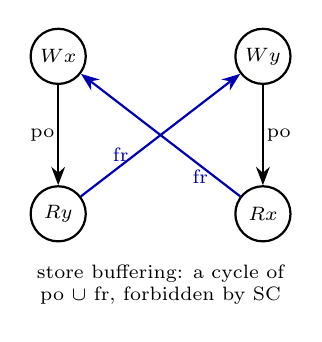
\begin{tikzpicture}[x=1cm,y=1cm]
      \node[ev] (w1) at (0,2) {\scriptsize $W x$};
      \node[ev] (r1) at (0,0) {\scriptsize $R y$};
      \node[ev] (w2) at (2.6,2) {\scriptsize $W y$};
      \node[ev] (r2) at (2.6,0) {\scriptsize $R x$};
      \draw[arr] (w1) -- node[lab,left]{po} (r1);
      \draw[arr] (w2) -- node[lab,right]{po} (r2);
      \draw[arr,blue!70!black] (r1) -- node[lab,pos=0.25,above]{fr} (w2);
      \draw[arr,blue!70!black] (r2) -- node[lab,pos=0.25,below]{fr} (w1);
      \node[font=\scriptsize,align=center] at (1.3,-0.9) {store buffering: a cycle of\\
        po $\cup$ fr, forbidden by SC};
    \end{tikzpicture}
  \end{column}
  \end{columns}
\end{frame}

%=====================================================================
\section{What is new compared to cvc5 main}

\begin{frame}{The changes at a glance}
  \scriptsize
  \begin{tabular}{@{}lL{11.2cm}@{}}
    \toprule
    component & change \\
    \midrule
    kinds, API & \new{\sm{RELATION\_CYCLIC}} (\sm{rel.cyclic}), \new{\sm{RELATION\_IS\_FUNCTIONAL}}
      (\sm{rel.is-functional}), \sm{RELATION\_RCLOSURE}, \sm{RELATION\_RTCLOSURE}
      (\sm{rel.rclosure}, \sm{rel.rtclosure}); parser, printer, CPC signature \\
    type rules & a binary relation whose columns have the same sort (cyclic, closures);
      any binary relation (functional) \\
    rewriter & evaluation and elimination rules (constants, empty set, singletons, unions) \\
    relations solver & \new{the calculus}: cycle witness, minimality, acyclicity, anchors,
      closure induction, functionality, lazy closure splits, grounding conflicts \\
    strategy & a new full-effort step, three last-call steps, \sm{needsCheckLastEffort} \\
    options & \sm{--rels-functional-mode}, \sm{--rels-acyclic-anchor},
      \sm{--rels-acyclic-backward-chords}, \sm{--rels-tc-subset}, \sm{--rels-tc-down-lazy},
      \sm{--rels-acyclic-hammer} \\
    defaults & MiniSat under \sm{--sets-exp} (justification heuristic), except for sygus-style problems \\
    fixes & closure rules (edge explanations, conclusions on the tuple of the explanation);
      no redundant facts in the sets solver \\
    tests, docs & 53 regression files; \sm{docs/theories/sets-and-relations.rst} \\
    \bottomrule
  \end{tabular}
  \medskip

  Against cvc5 main (a3f47bdffd): 28 source files, $+3305/-131$ lines; tests $+1958$ lines.\\
  \sm{scripts/} (experiment scripts, these slides) is temporary.
\end{frame}

\begin{frame}{New predicates}
  \begin{columns}[T]
  \begin{column}{0.5\textwidth}
    \begin{block}{\sm{(rel.cyclic R)}, \ $R$ : \sm{(Relation T T)}}
      \small
      \[ \cyc{R} \iff \exists x.\ (x,x)\in R^{+} \]
      Acyclicity is \sm{(not (rel.cyclic R))}.\\[1mm]
      e.g.\ \sm{(rel.cyclic (set.union R S))} holds for $R=\{(a,b)\}$, $S=\{(b,a)\}$;
      \sm{(rel.cyclic R)} and \sm{(rel.cyclic S)} do not.
    \end{block}
    \begin{block}{\sm{(rel.is-functional R)}, \ $R$ : \sm{(Relation T1 T2)}}
      \small
      \[ \fun{R} \iff \forall x\,y\,z.\ (x,y),(x,z)\in R \Rightarrow y=z \]
      Right-unique, not necessarily total.
    \end{block}
  \end{column}
  \begin{column}{0.48\textwidth}
    \begin{block}{\sm{(rel.rclosure R)}, \sm{(rel.rtclosure R)}}
      \small
      $R$ plus $(x,x)$ for every $x$ in its domain or range; and that union with
      $R^{+}$. Eliminated by rewriting when $R$ is built from $\emptyset$, singletons and
      unions; otherwise the solver answers \sm{unknown}.
    \end{block}
    \small
    \textbf{Why a predicate and not a definition?} The definitions need a quantifier (or the
    universe set, which cvc5 does not interpret as all elements). As predicates, the solver
    builds \emph{witnesses} and \emph{explanations} for them, and uses their structure
    (unions, closures, joins) in its rules.
  \end{column}
  \end{columns}
\end{frame}

\begin{frame}{Rewrite rules: what holds in every context}
  \small
  The rewriter only replaces a term by an \emph{equivalent} term, independently of the
  assertions:
  \begin{center}\scriptsize\setlength{\tabcolsep}{4pt}
  \begin{tabular}{@{}lll@{}}
    \toprule
    term & rewritten to & why \\
    \midrule
    \sm{(rel.cyclic $\emptyset$)} & \sm{false} & no pair at all \\
    \sm{(rel.cyclic \{(x,y)\})} & \sm{(= x y)} & only a self-loop \\
    \sm{(rel.cyclic $c$)}, $c$ constant & \sm{true} / \sm{false} & evaluate $c^{+}$ \\
    \midrule
    \sm{(rel.is-functional X)}, $X$: $\emptyset$, \sm{\{t\}}, \sm{(rel.iden A)} & \sm{true} & at most one image \\
    \sm{(rel.is-functional $c$)}, $c$ constant & \sm{true} / \sm{false} & first components \\
    \midrule
    \sm{(rel.rclosure \{(x,y)\})} & $\{(y,y)\}\cup(\{(x,x)\}\cup\{(x,y)\})$ & definition \\
    \sm{(rel.rclosure (set.union A B))} & \sm{(rel.rclosure A)} $\cup$ \sm{(rel.rclosure B)} & union \\
    \sm{(rel.rtclosure R)} & \sm{(rel.rclosure R)} $\cup$ \sm{(rel.tclosure R)} & definition \\
    \bottomrule
  \end{tabular}
  \end{center}
  Everything else is done by \emph{inference rules} in the relations solver (next section).
\end{frame}

%=====================================================================
\section{The calculus}

\begin{frame}{Notation}
  \begin{columns}[T]
  \begin{column}{0.55\textwidth}
    \small
    \begin{itemize}
      \item A configuration: the asserted literals and the equivalence classes of the
        equality engine; $t \sim t'$: equal in the current context.
      \item A rule
        \(\inferrule{P_1 \\ \dots \\ P_n}{C}\)
        sends the \emph{lemma} $P_1\wedge\dots\wedge P_n \Rightarrow C$, a valid clause whose
        premises are the explanation (used by conflict analysis, unsat cores and proofs).
      \item Fresh symbols are skolems, cached by their key, so each is created once.
      \item The \emph{cycle witness} of $\cyc{R_1\cup\dots\cup R_k}$: elements
        $s_1,\dots,s_l$ with $s_l = s_1$ ($l-1$ edges), each edge in some $\TC(R_j)$.
    \end{itemize}
  \end{column}
  \begin{column}{0.43\textwidth}
    \centering
    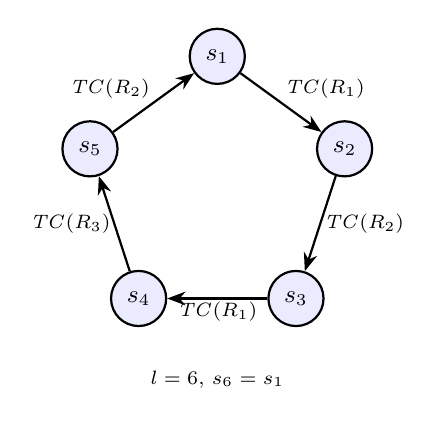
\begin{tikzpicture}
      \foreach \i/\a in {1/90,2/18,3/-54,4/-126,5/162} {
        \node[ev,fill=blue!8] (s\i) at (\a:1.7cm) {$s_{\i}$};
      }
      \draw[arr] (s1) -- node[lab,above right]{$\TC(R_1)$} (s2);
      \draw[arr] (s2) -- node[lab,right]{$\TC(R_2)$} (s3);
      \draw[arr] (s3) -- node[lab,below]{$\TC(R_1)$} (s4);
      \draw[arr] (s4) -- node[lab,left]{$\TC(R_3)$} (s5);
      \draw[arr] (s5) -- node[lab,above left]{$\TC(R_2)$} (s1);
      \node[font=\scriptsize] at (0,-2.4) {$l = 6$, $s_6 = s_1$};
    \end{tikzpicture}
  \end{column}
  \end{columns}
\end{frame}

\begin{frame}{Cyclicity: creating and unrolling the witness}
  \small\mprset{sep=1.2em}\vspace{-2mm}
  For an asserted $\cyc{R}$ (fresh $s$, $s_1$, $l$, $s_{i+1}$):
  \begin{mathpar}
    \inferrule*[right=\rn{Cycle-Def}]{\cyc{R} \\ R \text{ not a union}}{(s,s)\in \TC(R)}
    \and
    \inferrule*[right=\rn{Inst-Cycle}]{\cyc{R_1\cup\dots\cup R_k}}{1 < l}
    \\
    \inferrule*[right=\rn{Unroll}]{i < l}
      {(s_i,s_{i+1})\in \TC(R_1)\ \vee\ \dots\ \vee\ (s_i,s_{i+1})\in \TC(R_k)}
    \and
    \inferrule*[right=\rn{Split-Len}]{\cyc{R} \\ i \le l}{i < l\ \vee\ (l = i \wedge s_i = s_1)}
    \and
    \inferrule*[right=\rn{Same-Operands}]{\cyc{R'} \\ R' \text{ has the operands of } R}
      {\cyc{R}}
  \end{mathpar}
  \footnotesize
  \begin{itemize}
    \item The operands of nested unions are flattened: the witness of
      $\cyc{rf\cup(po\cup co)}$ alternates between $\TC(rf)$, $\TC(po)$, $\TC(co)$.
    \item One \rn{Unroll} per check round; at last call the witness is completed to the value
      of $l$ in the candidate model.
    \item \rn{Unroll} needs no $\cyc{R}$ premise: if $\cyc{R}$ is false, $l$ is unconstrained
      and $l \le 1$ makes every instance vacuous.
  \end{itemize}
\end{frame}

\begin{frame}{Minimality: the witness is a shortest cycle}
  \begin{columns}[T]
  \begin{column}{0.6\textwidth}
    \footnotesize\mprset{sep=1.2em}
    The witness can be a shortest cycle of $\TC(R_1)\cup\dots\cup\TC(R_k)$ ($q<r\le l$, every
    $R_j$):
    \begin{mathpar}
      \inferrule*[right=\rn{Alternate}]{\cyc{R} \\ i < l}
        {\neg\big((s_{i-1},s_i)\in\TC(R_j) \wedge (s_i,s_{i+1})\in\TC(R_j)\big)}
      \\
      \inferrule*[right=\rn{Alt-Close}]{\cyc{R} \\ l = i+1}
        {\neg\big((s_i,s_{i+1})\in\TC(R_j) \wedge (s_1,s_2)\in\TC(R_j)\big)}
      \\
      \inferrule*[right=\rn{Chord}]{\cyc{R} \\ r \le l \\ q < r-1}
        {(s_q,s_r)\notin\TC(R_j)}
      \and
      \inferrule*[right=\rn{Distinct}]{\cyc{R} \\ r \le l \\ (q,r)\ne(1,l)}{s_q \ne s_r}
    \end{mathpar}
    \textbf{\rn{Backward}} (\sm{--rels-acyclic-backward-chords}): $(s_r,s_q)\notin\TC(R_j)$ if it
    closes a shorter cycle; lets a totality axiom (e.g.\ $po$) bound the witness.
  \end{column}
  \begin{column}{0.38\textwidth}
    \centering
    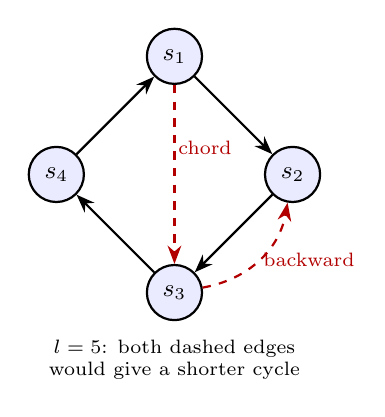
\begin{tikzpicture}
      \foreach \i/\a in {1/90,2/0,3/-90,4/180} {
        \node[ev,fill=blue!8] (s\i) at (\a:1.5cm) {$s_{\i}$};
      }
      \draw[arr] (s1) -- (s2);
      \draw[arr] (s2) -- (s3);
      \draw[arr] (s3) -- (s4);
      \draw[arr] (s4) -- (s1);
      \draw[arr,dashed,red!70!black] (s1) -- node[lab,right,pos=0.35]{chord} (s3);
      \draw[arr,dashed,red!70!black] (s3) to[bend right=35] node[lab,right]{backward} (s2);
      \node[font=\scriptsize,align=center] at (0,-2.35) {$l=5$: both dashed edges\\would give a shorter cycle};
    \end{tikzpicture}
  \end{column}
  \end{columns}
\end{frame}

\begin{frame}{Acyclicity}
  \small\vspace{-2mm}
  For an asserted $\neg\cyc{u}$:
  \begin{mathpar}
    \inferrule*[right=\rn{Acyclic-Down}]{(a,b)\in\TC(R) \\ \neg\cyc{u} \\ u \sim R}{a \ne b}
    \and
    \inferrule*[right=\rn{Register}]{\neg\cyc{u}}{u \subseteq \TC(u)}
  \end{mathpar}
  \begin{itemize}
    \item \rn{Acyclic-Down} turns every reflexive closure membership into a conflict. The
      existing closure rules produce those memberships:
      {\footnotesize
      \begin{mathpar}
        \inferrule*[right=\rn{TC-Up}]{(a,b)\in R \\ (b,c)\in \TC(R)}{(a,c)\in\TC(R)}
        \and
        \inferrule*[right=\rn{TC-Down}]{(a,b)\in\TC(R)}{(a,b)\in R \vee \big((a,k_1),(k_2,b)\in R
          \wedge (k_1 = k_2 \vee (k_1,k_2)\in\TC(R))\big)}
      \end{mathpar}}
    \item \rn{Register} is valid and does nothing logically: it makes $\TC(u)$ a term of the
      solver even if the input never mentions it, so that a cycle of $u$ is found.
    \item The conclusion is stated on the tuple of the explanation, not on its representative
      (the lemma is context-independent).
  \end{itemize}
\end{frame}

\begin{frame}{Cyclic meets acyclic: anchor rules}
  \begin{columns}[T]
  \begin{column}{0.6\textwidth}
    \small
    A cycle of $R$ all of whose edges lie in $\TC(S)$ would be a cycle of $S$:
    \begin{mathpar}
      \inferrule*[right=\rn{Inclusion}]{\cyc{R} \\ \neg\cyc{S}}
        {t\in R' \wedge t \notin \TC(S)}
      \\
      \inferrule*[right=\rn{Branch}]{\cyc{R} \\ \neg\cyc{S} \\ l = N}
        {\textstyle\bigvee_{i<N} (s_i,s_{i+1})\notin\TC(S)}
    \end{mathpar}
    $t$ fresh; $R'$: the operands of $R$ \emph{not} syntactically in $\TC(S)$ (e.g.\
    $S\cap Y$, $\TC(S)$, $S;S$ are). If there is none, the lemma is \sm{false}.
    \medskip

    \rn{Branch} is sent at last call, with $N$ the value of $l$ in the candidate model; with
    $l=N$ in its premises the listed edges are the whole cycle. \sm{--rels-acyclic-anchor}:
    \sm{branch} (default), \sm{inclusion}, \sm{both}, \sm{none}.
  \end{column}
  \begin{column}{0.38\textwidth}
    \centering
    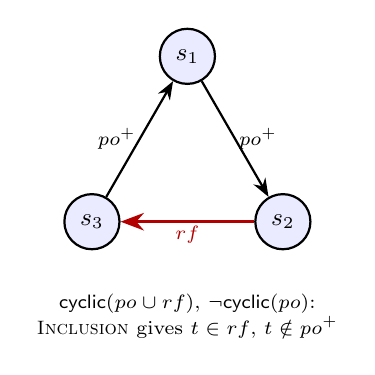
\begin{tikzpicture}
      \foreach \i/\a in {1/90,2/-30,3/210} {
        \node[ev,fill=blue!8] (s\i) at (\a:1.4cm) {$s_{\i}$};
      }
      \draw[arr] (s1) -- node[lab,right]{$po^{+}$} (s2);
      \draw[arr,very thick,red!70!black] (s2) -- node[lab,below]{$rf$} (s3);
      \draw[arr] (s3) -- node[lab,left]{$po^{+}$} (s1);
      \node[font=\scriptsize,align=center] at (0,-1.9)
        {$\cyc{po\cup rf}$, $\neg\cyc{po}$:\\\rn{Inclusion} gives $t\in rf$, $t\notin po^{+}$};
    \end{tikzpicture}
  \end{column}
  \end{columns}
\end{frame}

\begin{frame}{Closure induction (\sm{--rels-tc-subset})}
  \small
  $\TC(R)$ is the least transitive relation that contains $R$:
  \begin{mathpar}
    \inferrule*[right=\rn{TC-Subset}]{(a,b)\in\TC(R) \\ R\subseteq S \\ S;S\subseteq S}{(a,b)\in S}
  \end{mathpar}
  The transitive supersets $S$ recognised in the current context:
  \begin{center}\footnotesize
  \begin{tabular}{@{}L{4.6cm}L{3.9cm}L{5.4cm}@{}}
    \toprule
    superset $S$ & recognised by & example \\
    \midrule
    $\TC(X)$, $R$ syntactically in $\TC(X)$ & the shape of $R$ & $R = po^{+}\cap loc$, $S = po^{+}$ \\
    $S$ transitive, $R\subseteq S$ asserted & $(R\cup S) = S$ in the context &
      $S = A\times B$, a closure, $J;J^T$ with $\fun{J}$ \\
    $R$ itself & $(R;R)\subseteq R$ asserted & $co$ transitive: $\TC(co)=co$ \\
    $R$ itself & $R\subseteq A\times B$, $A\cap B=\emptyset$ & $fr$ from reads to writes: $\TC(fr)=fr$ \\
    $X$, transitive & $R = X\cap Y$ or $R = X\setminus Y$ & \\
    \bottomrule
  \end{tabular}
  \end{center}
  No fresh element: where it applies, one lemma replaces an unbounded descent of \rn{TC-Down}
  splits, each of which introduces two elements. This is what the hand proofs of the
  benchmarks use (``every $ghb$ path is in $po^{+}$'').
\end{frame}

\begin{frame}{Functionality (\sm{--rels-functional-mode})}
  \small
  \begin{mathpar}
    \inferrule*[right=\rn{Fun-UF}]{\fun{R} \\ (x,y)\in S \\ S\sim R}{y = f_R(x)}
    \and
    \inferrule*[right=\rn{Fun-Pairs}]{\fun{R} \\ (x_1,y_1)\in R \\ (x_2,y_2)\in R}{x_1 = x_2 \Rightarrow y_1 = y_2}
    \\
    \inferrule*[right=\rn{Not-Fun}]{\neg\fun{R}}{(k_1,k_2)\in R \wedge (k_1,k_3)\in R \wedge k_2\ne k_3}
  \end{mathpar}
  \begin{itemize}
    \item \sm{uf} (default): a fresh function $f_R$; linear in the members, congruence does the
      rest: $(a,b),(a,c)\in R$ give $b = f_R(a) = c$. \sm{pairs}: quadratic, no function symbol
      (used when the logic has no UF).
    \item Feeds closure induction: $J;J^T$ is transitive if $J$ is functional ($J^T;J$
      relates only equal elements), e.g.\ \emph{same location} $= address;address^T$.
  \end{itemize}
\end{frame}

\begin{frame}{Splitting closures and joins: eager, lazy, or not at all}
  \small
  \textbf{Eager} (cvc5 main): \rn{TC-Down} for every closure membership that the known members
  do not explain, and \rn{Join-Split} for every join membership, each with fresh elements. With
  finite model finding this floods the model with elements.
  {\footnotesize\mprset{sep=1.2em}
  \begin{mathpar}
    \inferrule*[right=\rn{Join-Split}]{(x,z)\in A;B}{(x,k)\in A \wedge (k,z)\in B}
    \and
    \inferrule*[right=\rn{Join-Compose}]{(x,y)\in A \\ (y,z)\in B}{(x,z)\in A;B}
  \end{mathpar}}

  \textbf{Lazy} (\sm{--rels-tc-down-lazy}): \rn{TC-Down} only at last call, and only for
  memberships that the known members of $R$ do not explain. Unsat proofs that never unfold a
  closure (closure induction) introduce no element.
  \medskip

  \textbf{Not at all} (\sm{--rels-acyclic-hammer}, for unsat problems): no \rn{TC-Down} and no
  \rn{Join-Split}. At last call, a closure or join membership that the known members do not
  explain is a conflict (\rn{Ground-TC}, \rn{Ground-Join}; see \emph{Grounding at last call}).
  \medskip

  Lazy and hammer move element introduction for closures and joins out of the full-effort
  check: the last call either introduces them only where needed (lazy) or refutes the
  candidate model instead (hammer).
\end{frame}

\begin{frame}{Why inference rules and not rewrite rules?}
  \footnotesize
  \begin{columns}[T]
  \begin{column}{0.4\textwidth}
    \begin{block}{The rewriter}
      maps a term to an \emph{equivalent} term:
      \begin{itemize}
        \item the same in every context (no access to assertions or to the model);
        \item no fresh symbols, no case splits;
        \item terminating, and applied to the input and to every lemma.
      \end{itemize}
      It gets the rules on the term alone: $\cyc{\emptyset}=\bot$,
      $\cyc{\{(x,y)\}} = (x=y)$, constants, closure elimination.
    \end{block}
    Rewriting $\cyc{R}$ to its definition needs a quantifier, or
    $\TC(R)\cap\mathit{iden}(\mathit{univ})\ne\emptyset$, which is wrong in cvc5 (the universe
    is not all elements) and hides the structure the rules use.
  \end{column}
  \begin{column}{0.58\textwidth}
    \scriptsize
    \begin{tabular}{@{}L{3.0cm}L{5.0cm}@{}}
      \toprule
      the rules need & e.g. \\
      \midrule
      a \textbf{witness} (an existential: fresh symbols) & \rn{Cycle-Def}, \rn{Inst-Cycle},
        \rn{Unroll}, \rn{Inclusion}, \rn{Not-Fun} \\
      \textbf{case splits} for the SAT solver & \rn{Unroll} picks an operand,
        \rn{Split-Len} continues or closes \\
      \textbf{other asserted facts} & \rn{TC-Subset} ($R\subseteq S$, $S$ transitive),
        anchors ($\cyc{R}$ and $\neg\cyc{S}$), \rn{Fun-UF} (a membership) \\
      \textbf{equivalence classes} & $S \sim R$, $u\sim R$: premises that hold now, not always \\
      \textbf{the candidate model} & \rn{Branch} ($l = N$), \rn{Ground-TC}, \rn{Ground-Join} \\
      \textbf{unbounded} unfolding & a witness of any length, one element per round \\
      \bottomrule
    \end{tabular}
  \end{column}
  \end{columns}
\end{frame}

\begin{frame}{Soundness}
  \small
  \begin{itemize}
    \item \textbf{Valid lemmas}, consequences of the definitions and the premises: the closure
      rules, \rn{Acyclic-Down}, \rn{Register}, \rn{TC-Subset}, \rn{Fun-Pairs}, and the grounding
      conflicts (their premises contain $S = \TC(R)$ or $S = A;B$ and the disequalities that
      block every derivation).
    \item \textbf{Lemmas about skolems}, satisfiability-preserving: any model of the input
      extends to one in which the witness is a shortest cycle of the operands' closures,
      $f_R$ maps every element to its image, etc. This covers \rn{Cycle-Def}, \rn{Inst-Cycle},
      \rn{Unroll}, \rn{Split-Len}, \rn{Alternate}, \rn{Alt-Close}, \rn{Chord}, \rn{Distinct},
      \rn{Backward}, \rn{Inclusion}, \rn{Fun-UF}, \rn{Not-Fun}. \rn{Branch} follows from them
      (thanks to $l = N$). The last call sends instances of the same rules (see \emph{Is
      introducing elements at last call sound?}).
    \item \textbf{Incompleteness is reported}, so cvc5 answers \sm{unknown} instead of a wrong
      \sm{sat}, when
      \begin{itemize}
        \item the length of a witness has no practical value in the model;
        \item a \sm{rel.rclosure} term is not eliminated by rewriting.
      \end{itemize}
    \item \textbf{Proofs.} The lemmas are trusted theory lemmas; their CPC proofs check with
      ethos (\sm{rel.cyclic}, \sm{rel.is-functional} are in the CPC signature).
  \end{itemize}
\end{frame}

%=====================================================================
\section{Strategy}

\begin{frame}{Where the rules run: cvc5's DPLL($T$) loop}
  \centering
  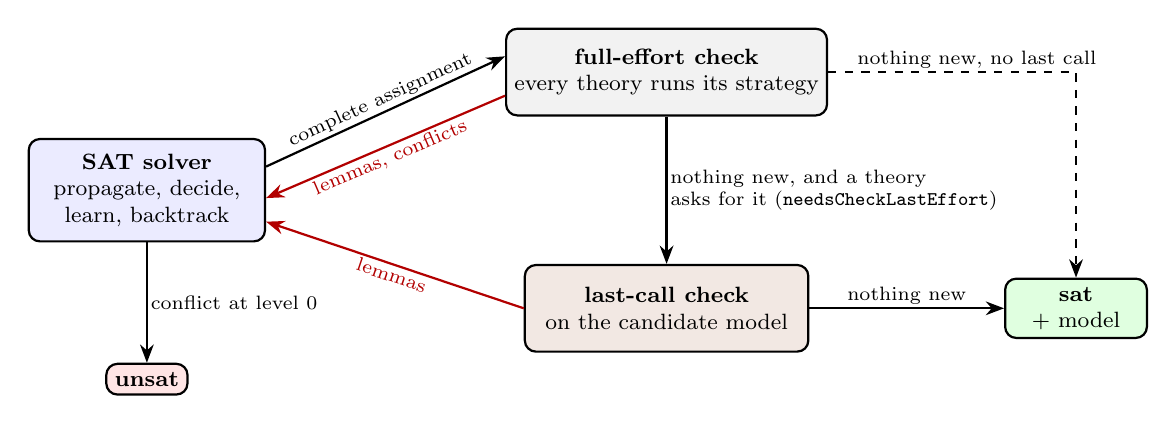
\begin{tikzpicture}
    \node[box,fill=blue!8,minimum width=3.0cm,minimum height=1.3cm] (sat) at (0,0)
      {\textbf{SAT solver}\\propagate, decide,\\learn, backtrack};
    \node[box,fill=gray!10,minimum width=3.6cm,minimum height=1.1cm] (full) at (6.6,1.5)
      {\textbf{full-effort check}\\every theory runs its strategy};
    \node[box,fill=lcc!12,minimum width=3.6cm,minimum height=1.1cm] (last) at (6.6,-1.5)
      {\textbf{last-call check}\\on the candidate model};
    \node[box,fill=green!12,minimum width=1.8cm] (model) at (11.8,-1.5) {\textbf{sat}\\+ model};
    \node[box,fill=red!10] (unsat) at (0,-2.4) {\textbf{unsat}};
    \draw[arr] ([yshift=3mm]sat.east) -- node[lab,above,sloped]{complete assignment}
      ([yshift=2mm]full.west);
    \draw[arr,red!70!black] ([yshift=-3mm]full.west) -- node[lab,below,sloped]{lemmas, conflicts}
      ([yshift=-1mm]sat.east);
    \draw[arr] (full.south) -- node[lab,right,align=left]{nothing new, and a theory\\
      asks for it (\sm{needsCheckLastEffort})} (last.north);
    \draw[arr,red!70!black] (last.west) -- node[lab,below,sloped]{lemmas} ([yshift=-4mm]sat.east);
    \draw[arr] (last.east) -- node[lab,above]{nothing new} (model.west);
    \draw[arr,dashed] (full.east) -| node[lab,above,pos=0.3]{nothing new, no last call}
      (model.north);
    \draw[arr] (sat.south) -- node[lab,right]{conflict at level 0} (unsat.north);
  \end{tikzpicture}
  \medskip

  \small
  \begin{itemize}
    \item The sets theory asks for a last call (\sm{needsCheckLastEffort}) if a cycle witness
      exists, or under \sm{--rels-tc-down-lazy} / \sm{--rels-acyclic-hammer} if closures or
      joins occur.
    \item Lemmas are permanent clauses; the witness and the caches are rolled back on
      backtracking (context-dependent).
  \end{itemize}
\end{frame}

\begin{frame}{The sets strategy at full effort}
  \centering
  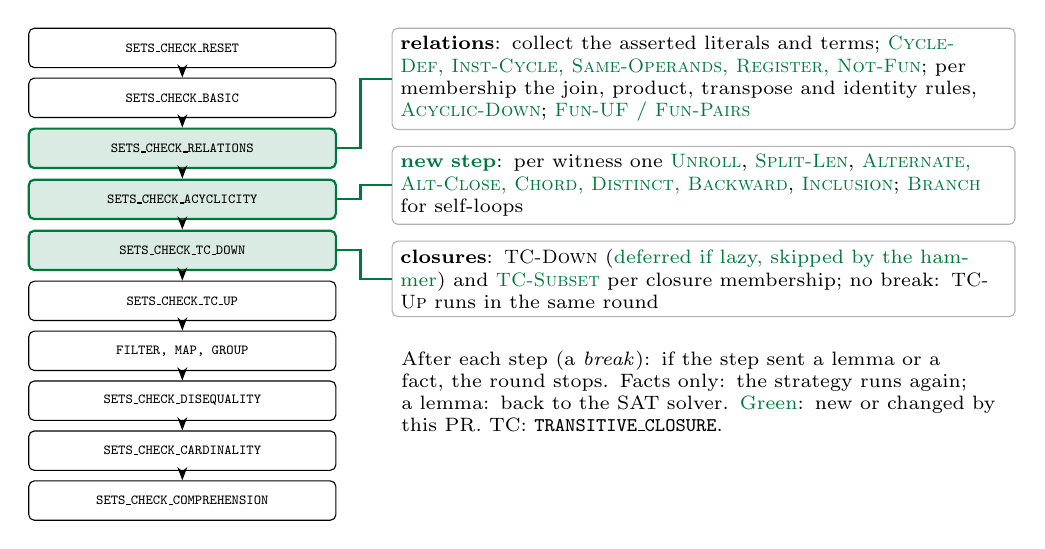
\begin{tikzpicture}[node distance=1.2mm]
    \tikzset{stp/.append style={minimum width=3.9cm,font=\tiny\ttfamily}}
    \node[stp] (reset) {SETS\_CHECK\_RESET};
    \node[stp,below=of reset] (basic) {SETS\_CHECK\_BASIC};
    \node[newstp,below=of basic] (rel) {SETS\_CHECK\_RELATIONS};
    \node[newstp,below=of rel] (acyc) {SETS\_CHECK\_ACYCLICITY};
    \node[newstp,below=of acyc] (down) {SETS\_CHECK\_TC\_DOWN};
    \node[stp,below=of down] (up) {SETS\_CHECK\_TC\_UP};
    \node[stp,below=of up] (fmg) {FILTER, MAP, GROUP};
    \node[stp,below=of fmg] (dis) {SETS\_CHECK\_DISEQUALITY};
    \node[stp,below=of dis] (card) {SETS\_CHECK\_CARDINALITY};
    \node[stp,below=of card] (comp) {SETS\_CHECK\_COMPREHENSION};
    \foreach \a/\b in {reset/basic,basic/rel,rel/acyc,acyc/down,down/up,up/fmg,fmg/dis,dis/card,card/comp} {
      \draw[->,>=Stealth] (\a) -- (\b);
    }
    \node[rules,anchor=north west,text width=7.7cm] (rrel) at ($(reset.north east)+(7mm,0)$)
      {\textbf{relations}: collect the asserted literals and terms; \new{\rn{Cycle-Def},
       \rn{Inst-Cycle}, \rn{Same-Operands}, \rn{Register}, \rn{Not-Fun}}; per membership the join,
       product, transpose and identity rules, \new{\rn{Acyclic-Down}}; \new{\rn{Fun-UF} /
       \rn{Fun-Pairs}}};
    \node[rules,text width=7.7cm,below=2mm of rrel.south west,anchor=north west] (racyc)
      {\textbf{\new{new step}}: per witness one \new{\rn{Unroll}}, \new{\rn{Split-Len}},
       \new{\rn{Alternate}, \rn{Alt-Close}, \rn{Chord}, \rn{Distinct}, \rn{Backward}},
       \new{\rn{Inclusion}};
       \new{\rn{Branch}} for self-loops};
    \node[rules,text width=7.7cm,below=2mm of racyc.south west,anchor=north west] (rdown)
      {\textbf{closures}: \rn{TC-Down} (\new{deferred if lazy, skipped by the hammer}) and
       \new{\rn{TC-Subset}} per closure membership; no break: \rn{TC-Up} runs in the same round};
    \draw[newc,thick] (rel.east) -- ++(3mm,0) |- (rrel.west);
    \draw[newc,thick] (acyc.east) -- ++(3mm,0) |- (racyc.west);
    \draw[newc,thick] (down.east) -- ++(3mm,0) |- (rdown.west);
    \node[font=\scriptsize,align=left,anchor=north west,text width=7.7cm] at ($(rdown.south west)+(0,-3mm)$)
      {After each step (a \emph{break}): if the step sent a lemma or a fact, the round stops.
       Facts only: the strategy runs again; a lemma: back to the SAT solver.
       \new{Green}: new or changed by this PR. TC: \sm{TRANSITIVE\_CLOSURE}.};
  \end{tikzpicture}
\end{frame}

\begin{frame}{Last call: the candidate model decides}
  \centering
  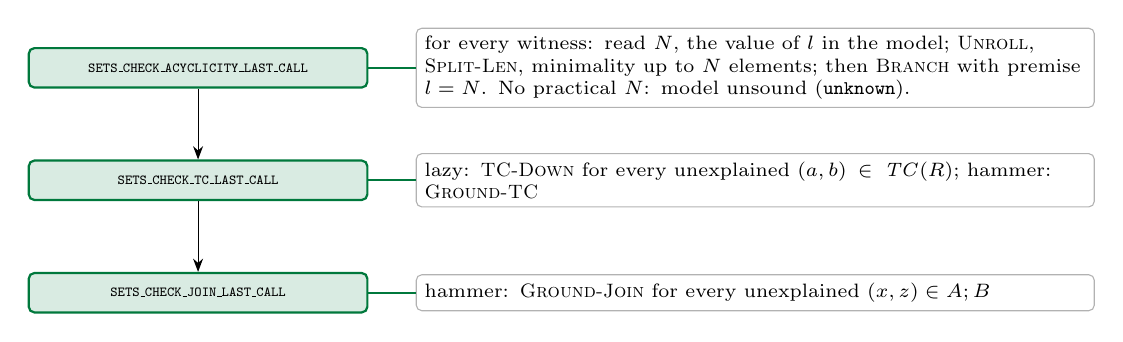
\begin{tikzpicture}[node distance=9mm]
    \tikzset{stp/.append style={font=\tiny\ttfamily}}
    \node[newstp,minimum width=4.3cm] (a) {SETS\_CHECK\_ACYCLICITY\_LAST\_CALL};
    \node[newstp,minimum width=4.3cm,below=of a] (t) {SETS\_CHECK\_TC\_LAST\_CALL};
    \node[newstp,minimum width=4.3cm,below=of t] (j) {SETS\_CHECK\_JOIN\_LAST\_CALL};
    \draw[->,>=Stealth] (a) -- (t);
    \draw[->,>=Stealth] (t) -- (j);
    \node[rules,right=6mm of a,text width=8.4cm] (ra)
      {for every witness: read $N$, the value of $l$ in the model; \rn{Unroll}, \rn{Split-Len},
       minimality up to $N$ elements; then \rn{Branch} with premise $l = N$. No practical $N$:
       model unsound (\sm{unknown}).};
    \node[rules,right=6mm of t,text width=8.4cm] (rt)
      {lazy: \rn{TC-Down} for every unexplained $(a,b)\in\TC(R)$; hammer: \rn{Ground-TC}};
    \node[rules,right=6mm of j,text width=8.4cm] (rj)
      {hammer: \rn{Ground-Join} for every unexplained $(x,z)\in A;B$};
    \draw[newc,thick] (a) -- (ra);
    \draw[newc,thick] (t) -- (rt);
    \draw[newc,thick] (j) -- (rj);
  \end{tikzpicture}
  \bigskip

  \small
  \begin{itemize}
    \item A step that sends a lemma ends the check; the SAT solver continues with it.
    \item Model-dependent rules belong here: at full effort the length of the witness is still
      symbolic, and the members of a relation are not final.
  \end{itemize}
\end{frame}

\begin{frame}{A cycle witness across the search}
  \centering
  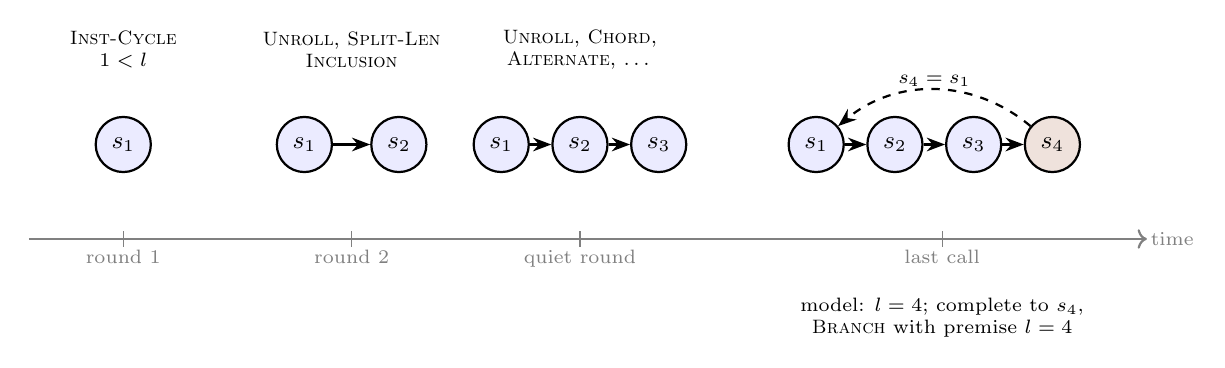
\begin{tikzpicture}[x=1cm,y=1cm]
    \draw[->,thick,gray] (0,0) -- (14.2,0) node[right,lab]{time};
    \foreach \x/\t in {1.2/round 1,4.1/round 2,7.0/quiet round,11.6/last call} {
      \draw[gray] (\x,0.1) -- (\x,-0.1) node[below,lab]{\t};
    }
    % round 1
    \node[ev,fill=blue!8] (a1) at (1.2,1.2) {$s_1$};
    \node[lab,align=center] at (1.2,2.4) {\rn{Inst-Cycle}\\$1<l$};
    % round 2
    \node[ev,fill=blue!8] (b1) at (3.5,1.2) {$s_1$};
    \node[ev,fill=blue!8] (b2) at (4.7,1.2) {$s_2$};
    \draw[arr] (b1) -- (b2);
    \node[lab,align=center] at (4.1,2.4) {\rn{Unroll}, \rn{Split-Len}\\\rn{Inclusion}};
    % round 3
    \node[ev,fill=blue!8] (c1) at (6.0,1.2) {$s_1$};
    \node[ev,fill=blue!8] (c2) at (7.0,1.2) {$s_2$};
    \node[ev,fill=blue!8] (c3) at (8.0,1.2) {$s_3$};
    \draw[arr] (c1) -- (c2);
    \draw[arr] (c2) -- (c3);
    \node[lab,align=center] at (7.0,2.4) {\rn{Unroll}, \rn{Chord},\\\rn{Alternate}, \dots};
    % last call
    \node[ev,fill=blue!8] (d1) at (10.0,1.2) {$s_1$};
    \node[ev,fill=blue!8] (d2) at (11.0,1.2) {$s_2$};
    \node[ev,fill=blue!8] (d3) at (12.0,1.2) {$s_3$};
    \node[ev,fill=lcc!15] (d4) at (13.0,1.2) {$s_4$};
    \draw[arr] (d1) -- (d2);
    \draw[arr] (d2) -- (d3);
    \draw[arr] (d3) -- (d4);
    \draw[arr,dashed] (d4) to[bend right=40] node[lab,above]{$s_4 = s_1$} (d1);
    \node[lab,align=center] at (11.6,-1.0) {model: $l = 4$; complete to $s_4$,\\\rn{Branch} with premise $l=4$};
  \end{tikzpicture}
  \bigskip

  \small
  \begin{itemize}
    \item Each round's lemmas go back to the SAT solver; a conflict may backtrack past the
      creation of $s_3$, which then disappears from the witness. It is recreated, as the same
      skolem, with lemmas that are already known: that round is quiet, and the last call runs.
    \item A witness that is too long for the problem is refuted by minimality and the anchors;
      a short one survives and its edges become the model's cycle.
  \end{itemize}
\end{frame}

%=====================================================================
\section{Last call and model construction}

\begin{frame}{Last call: completing the witness}
  \begin{columns}[T]
  \begin{column}{0.52\textwidth}
    \begin{algorithm}[H]
      \caption{\sm{checkAcyclicityLastCall}}
      \ForEach{witness $s_1..s_c$, $l$ of an asserted $\cyc{R_1\cup\dots\cup R_k}$}{
        $N \leftarrow$ the value of $l$ in the candidate model\;
        \If{$N$ is not a constant, or $N > 10000$}{
          \rn{Len-Unknown}: model unsound; \textbf{continue}\;
        }
        \While{$c < N$}{
          $s_{c+1} \leftarrow$ the skolem cached for $(R,\ c+1)$\;
          send \rn{Unroll}$_c$, \rn{Alternate}$_c$, \rn{Alt-Close}$_c$\;
          $c \leftarrow c+1$\;
          send \rn{Split-Len}$_c$, and \rn{Chord}, \rn{Distinct},\\
          \quad \rn{Backward} for the pairs up to $s_c$\;
        }
        \If{$N \ge 2$}{
          \ForEach{asserted $\neg\cyc{S}$}{
            send \rn{Branch}$_N$ (once per $R$, $S$, $N$)\;
          }
        }
      }
    \end{algorithm}
    \scriptsize A lemma that was sent before is not sent again (the lemma cache survives
    backtracking).
  \end{column}
  \begin{column}{0.46\textwidth}
    \centering
    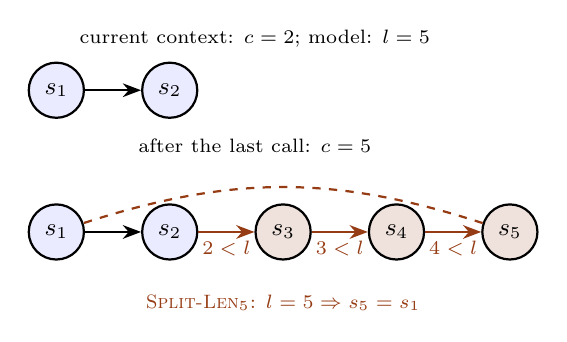
\begin{tikzpicture}[x=1.2cm,y=1cm]
      \node[lab] at (2.1,1.9) {current context: $c = 2$; model: $l = 5$};
      \node[ev,fill=blue!8] (a1) at (0,1.25) {$s_1$};
      \node[ev,fill=blue!8] (a2) at (1.2,1.25) {$s_2$};
      \draw[arr] (a1) -- (a2);
      \node[lab] at (2.1,0.55) {after the last call: $c = 5$};
      \node[ev,fill=blue!8] (b1) at (0,-0.55) {$s_1$};
      \node[ev,fill=blue!8] (b2) at (1.2,-0.55) {$s_2$};
      \node[ev,fill=lcc!15] (b3) at (2.4,-0.55) {$s_3$};
      \node[ev,fill=lcc!15] (b4) at (3.6,-0.55) {$s_4$};
      \node[ev,fill=lcc!15] (b5) at (4.8,-0.55) {$s_5$};
      \draw[arr] (b1) -- (b2);
      \draw[arr,lcc] (b2) -- node[lab,below=2pt]{$2<l$} (b3);
      \draw[arr,lcc] (b3) -- node[lab,below=2pt]{$3<l$} (b4);
      \draw[arr,lcc] (b4) -- node[lab,below=2pt]{$4<l$} (b5);
      \draw[dashed,thick,lcc] (b5) to[bend right=18] (b1);
      \node[lab,lcc] at (2.4,-1.45) {\rn{Split-Len}$_5$: $l=5 \Rightarrow s_5 = s_1$};
    \end{tikzpicture}
    \medskip

    \footnotesize
    \begin{itemize}
      \item \textbf{Why $c < N$}: full effort adds one element per round, backtracking removes
        them. Re-unrolled with the same skolems, a round sends only known lemmas: it is quiet,
        and the last call runs. Each new edge (orange) has its own guard $i < l$.
    \end{itemize}
  \end{column}
  \end{columns}
\end{frame}

\begin{frame}{The lemmas about the witness}
  \footnotesize\vspace{-1mm}
  Each lemma is \emph{premise} $\Rightarrow$ \emph{conclusion}, for the witness of
  $\cyc{R}$, $R = R_1\cup\dots\cup R_k$, and every operand $R_j$:
  \begin{center}
  \scriptsize\renewcommand{\arraystretch}{1.05}
  \begin{tabular}{@{}L{2.4cm}L{4.6cm}L{7.2cm}@{}}
    \toprule
    rule & premise & conclusion \\
    \midrule
    \rn{Inst-Cycle} & $\cyc{R}$ & $1 < l$ \\
    \rn{Unroll}$_i$ & $i < l$ & $(s_i,s_{i+1})\in\TC(R_1)\vee\dots\vee(s_i,s_{i+1})\in\TC(R_k)$ \\
    \rn{Split-Len}$_r$ & $\cyc{R}\wedge r \le l$ & $r < l\ \vee\ (l = r \wedge s_r = s_1)$ \\
    \rn{Alternate}$_i$ & $\cyc{R}\wedge i < l$ \hfill ($i\ge 2$) &
      $\neg\big((s_{i-1},s_i)\in\TC(R_j)\wedge(s_i,s_{i+1})\in\TC(R_j)\big)$ \\
    \rn{Alt-Close}$_i$ & $\cyc{R}\wedge l = i+1$ \hfill ($i\ge 2$) &
      $\neg\big((s_i,s_{i+1})\in\TC(R_j)\wedge(s_1,s_2)\in\TC(R_j)\big)$ \\
    \rn{Chord}$_{q,r}$ & $\cyc{R}\wedge r\le l$ \hfill ($q < r-1$) & $(s_q,s_r)\notin\TC(R_j)$ \\
    \rn{Distinct}$_{q,r}$ & $\cyc{R}\wedge r\le l\ [{}\wedge r\ne l$ if $q=1]$ & $s_q\ne s_r$ \\
    \rn{Branch}$_N$ & $\cyc{R}\wedge\neg\cyc{S}\wedge \alert{l = N}$ &
      $(s_1,s_2)\notin\TC(S)\vee\dots\vee(s_{N-1},s_N)\notin\TC(S)$ \\
    \rn{Len-Unknown} & $l$ has no value $\le 10000$ & model unsound: \sm{unknown}, never \sm{sat} \\
    \bottomrule
  \end{tabular}
  \end{center}
  \begin{itemize}
    \item The premises mention the term $l$, never its value. $N$ only decides \emph{how many}
      instances the last call sends, and appears only as the literal $l = N$ of \rn{Branch}$_N$.
    \item $s_i$ is the skolem cached for $(R, i)$: full effort and the last call build the same
      element and lemma. The last call changes \emph{when} a lemma is sent, not \emph{what} it
      says.
  \end{itemize}
\end{frame}

\begin{frame}{Is introducing elements at last call sound? (1/2)}
  \begin{columns}[T]
  \begin{column}{0.53\textwidth}
    \small
    \textbf{Claim}: every model $M$ of the input extends to a model $M'$ that satisfies the
    lemmas about the witness \emph{for all indices and all $N$ at once}: whatever values of
    $l$ the candidate models show, no model of the input is lost (no wrong \sm{unsat}).
    \medskip

    $M'$ interprets only the skolems:
    \begin{itemize}
      \item $\cyc{R}$ true in $M$: take a \emph{shortest} cycle of
        $\TC(R_1)\cup\dots\cup\TC(R_k)$ in $M$, with $L-1$ edges. Set $l := L$, put
        $s_1,\dots,s_L$ along the cycle ($s_L = s_1$), and let $s_i$, $i > L$, be any element.
      \item $\cyc{R}$ false in $M$: $l := 1$, every $s_i$ any element.
    \end{itemize}
    Every guard of an index beyond $L$ ($i < l$, $r \le l$, $l = N$) is false in $M'$: the
    elements created for a larger value of $l$ are unconstrained.
  \end{column}
  \begin{column}{0.45\textwidth}
    \centering
    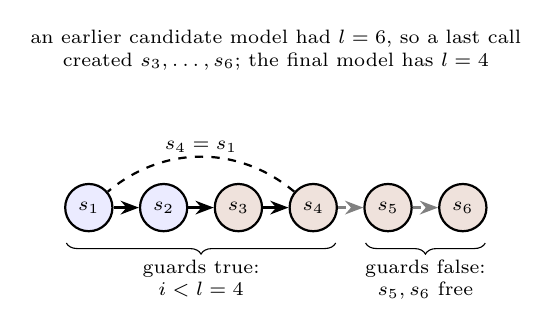
\begin{tikzpicture}[x=0.95cm,y=1cm]
      \node[lab,align=center] at (3.5,2.0) {an earlier candidate model had $l = 6$, so a
        last call\\created $s_3,\dots,s_6$; the final model has $l = 4$};
      \foreach \i in {1,2} {
        \node[ev,fill=blue!8,minimum size=6mm] (s\i) at (\i,0) {\scriptsize $s_{\i}$};
      }
      \foreach \i in {3,...,6} {
        \node[ev,fill=lcc!15,minimum size=6mm] (s\i) at (\i,0) {\scriptsize $s_{\i}$};
      }
      \foreach \i/\j in {1/2,2/3,3/4} { \draw[arr] (s\i) -- (s\j); }
      \draw[arr,dashed,gray] (s4) -- (s5);
      \draw[arr,dashed,gray] (s5) -- (s6);
      \draw[dashed,thick] (s4) to[bend right=40] node[lab,above]{$s_4 = s_1$} (s1);
      \draw[decorate,decoration={brace,mirror,amplitude=4pt}] (0.7,-0.45) -- (4.3,-0.45)
        node[midway,below=5pt,lab,align=center]{guards true:\\$i < l = 4$};
      \draw[decorate,decoration={brace,mirror,amplitude=4pt}] (4.7,-0.45) -- (6.3,-0.45)
        node[midway,below=5pt,lab,align=center]{guards false:\\$s_5, s_6$ free};
    \end{tikzpicture}
    \bigskip

    \footnotesize
    \begin{itemize}
      \item A shortest cycle exists if a cycle does; no edge of a $\TC(R_j)$ shortcuts it.
      \item Other rules on the $s_i$ (\rn{TC-Down}, \dots) are valid or pick their own fresh
        elements after the $s_i$.
    \end{itemize}
  \end{column}
  \end{columns}
\end{frame}

\begin{frame}{Is introducing elements at last call sound? (2/2)}
  \footnotesize
  Every lemma holds in $M'$ ($\cyc{R}$ true in $M$, shortest cycle with $L-1$ edges,
  $G = \TC(R_1)\cup\dots\cup\TC(R_k)$):
  \begin{center}
  \scriptsize\renewcommand{\arraystretch}{1.1}
  \begin{tabular}{@{}L{2.3cm}L{8.8cm}L{3.0cm}@{}}
    \toprule
    rule & index up to $L$: the guard holds, the conclusion too & index beyond $L$ \\
    \midrule
    \rn{Inst-Cycle} & $1 < L$: the cycle has an edge & --- \\
    \rn{Unroll}$_i$ & $i < L$: $(s_i,s_{i+1})$ is an edge of the cycle, so it is in some
      $\TC(R_j)$ & $i < l$ false \\
    \rn{Split-Len}$_r$ & $r < L$: $r < l$; \ $r = L$: $l = L$ and $s_L = s_1$ & $r \le l$ false \\
    \rn{Alternate}$_i$, \rn{Alt-Close}$_i$ & two consecutive edges in $\TC(R_j)$ give, by
      transitivity, one edge of $\TC(R_j)$: a cycle of $G$ with one edge less & $i<l$,
      $l=i+1$ false \\
    \rn{Chord}$_{q,r}$ & $(s_q,s_r)\in\TC(R_j)$ skips $r-q\ge 2$ edges: a shorter cycle (for
      $(1,L)$: a self-loop, 1 edge) & $r \le l$ false \\
    \rn{Distinct}$_{q,r}$ & $s_q = s_r$ closes the cycle $s_q..s_r$ of $r-q < L-1$ edges & $r \le l$
      false \\
    \rn{Branch}$_N$ & $N \ne L$: $l = N$ is false. $N = L$: if every edge were in $\TC(S)$,
      $S$ would be cyclic in $M$, but $M \models \neg\cyc{S}$ & --- \\
    \bottomrule
  \end{tabular}
  \end{center}
  \textbf{$\cyc{R}$ false in $M$}: every premise contains $\cyc{R}$, except \rn{Unroll}$_i$, whose
  guard $i < l = 1$ is false.
  \medskip

  \textbf{The other direction} (no wrong \sm{sat}): a quiet last call means that the model
  satisfies \rn{Unroll}$_1..$\rn{Unroll}$_{N-1}$ and \rn{Split-Len}$_N$ with $l = N$: it has a
  cycle (see \emph{Model construction}). Without a practical $N$: \sm{unknown}.
\end{frame}

\begin{frame}{Grounding at last call: the algorithm}
  \begin{columns}[T]
  \begin{column}{0.54\textwidth}
    \begin{algorithm}[H]
      \caption{last call: closures, joins}
      collect the members of every relation, by representatives\;
      \ForEach{membership $(a,b)\in\TC(R)$}{
        \If{no path $a\to\dots\to b$ in the graph of the known members of $R$}{
          \lIf{lazy}{send \rn{TC-Down} for $(a,b)$}
          \lElse{send \rn{Ground-TC} \hfill (hammer)}
        }
      }
      \If{hammer}{
        \ForEach{membership $(x,z)\in A;B$}{
          \If{no known $(x,y)\in A$ with $(y,z)\in B$}{
            send \rn{Ground-Join}\;
          }
        }
      }
    \end{algorithm}
    \footnotesize
    \begin{itemize}
      \item Closure (\sm{isTCReachable}): depth-first search from $a$ over the members of
        $R$ only.
      \item Join (\sm{isJoinReachable}): for each known $(x,y)\in A$, look up $(y,z)$ in the
        membership trie of $B$.
    \end{itemize}
  \end{column}
  \begin{column}{0.44\textwidth}
    \centering
    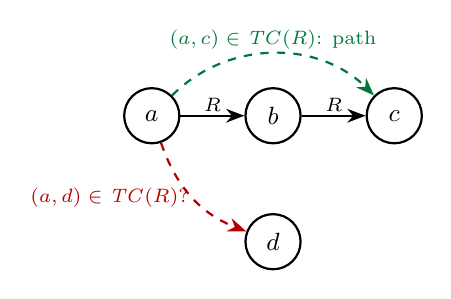
\begin{tikzpicture}[x=1.1cm,y=1cm]
      \node[ev] (a) at (0,0) {$a$};
      \node[ev] (b) at (1.4,0) {$b$};
      \node[ev] (c) at (2.8,0) {$c$};
      \node[ev] (d) at (1.4,-1.6) {$d$};
      \draw[arr] (a) -- node[lab,above]{$R$} (b);
      \draw[arr] (b) -- node[lab,above]{$R$} (c);
      \draw[arr,dashed,newc] (a) to[bend left=45] node[lab,above]{$(a,c)\in\TC(R)$: path} (c);
      \draw[arr,dashed,red!70!black] (a) to[bend right=25] node[lab,left]{$(a,d)\in\TC(R)$?} (d);
    \end{tikzpicture}
    \medskip

    \footnotesize
    \raggedright
    $R = \{(a,b),(b,c)\}$: $(a,c)$ is explained, $(a,d)$ is not.
    \begin{itemize}
      \item lazy: \rn{TC-Down} adds $(a,k_1),(k_2,d)\in R$, \dots;
      \item hammer: \rn{Ground-TC} refutes this model: the SAT solver must change $R$, an
        equality, or the membership.
    \end{itemize}
  \end{column}
  \end{columns}
\end{frame}

\begin{frame}{Grounding conflict: \rn{Ground-Join}}
  \small\mprset{sep=1.2em}
  \begin{mathpar}
    \inferrule*[right=\rn{Ground-Join}]
      {(x,z)\in S \\ S = A;B \\
       A = \{(x_1,y_1),..,(x_n,y_n)\} \\ B = \{(u_1,z_1),..,(u_m,z_m)\} \\\\
       x_i\neq x \;\lor\; y_i\neq u_j \;\lor\; z_j\neq z \quad\text{for all } i, j}
      {\bot}
  \end{mathpar}
  \centering no pair of members composes to $(x,z)$
  \medskip

  \begin{columns}[T]
  \begin{column}{0.42\textwidth}
    \centering
    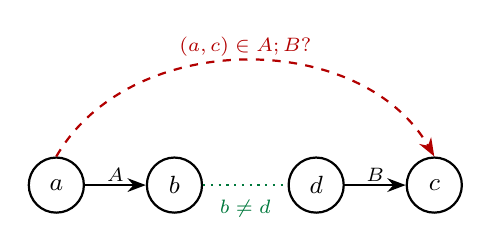
\begin{tikzpicture}[x=1cm,y=1cm]
      \node[ev] (a) at (0,0) {$a$};
      \node[ev] (b) at (1.5,0) {$b$};
      \node[ev] (d) at (3.3,0) {$d$};
      \node[ev] (c) at (4.8,0) {$c$};
      \draw[arr] (a) -- node[lab,above]{$A$} (b);
      \draw[arr] (d) -- node[lab,above]{$B$} (c);
      \draw[thick,dotted,newc] (b) -- (d) node[midway,below=4pt,lab,text=newc]{$b \neq d$};
      \draw[arr,dashed,red!70!black] (a.north) to[out=60,in=120] node[lab,above]{$(a,c)\in A;B$?} (c.north);
    \end{tikzpicture}
  \end{column}
  \begin{column}{0.56\textwidth}
    \footnotesize
    $(a,c)\in A;B$, $A = \{(a,b)\}$, $B = \{(d,c)\}$: one pair,
    \[ \underbrace{a\neq a}_{\text{false}} \;\lor\; \new{b\neq d} \;\lor\; \underbrace{c\neq c}_{\text{false}} \]
    The lemma keeps one true disjunct per pair:
    \[ \neg\big((a,c)\in S \land S = A;B \land A = \{(a,b)\} \land B = \{(d,c)\} \land \new{b\neq d}\big) \]
    Before: $\mathit{distinct}(a,b,c,d)$; every merge of two other elements (e.g.\ $a = c$)
    needed a new conflict (12 instead of 1).
  \end{column}
  \end{columns}
\end{frame}

\begin{frame}{Grounding conflict: \rn{Ground-TC}}
  \small\mprset{sep=1.2em}
  \begin{mathpar}
    \inferrule*[right=\rn{Ground-TC}]
      {(x,z)\in S \\ S = \TC(R) \\ R = \{(p_1,q_1),..,(p_n,q_n)\} \\\\
       p_i\notin U \;\lor\; (q_i\in U \land q_i\neq z) \quad\text{for all } i}
      {\bot}
  \end{mathpar}
  \vspace{-1mm}
  \centering
  \begin{tabular}{@{}l@{\quad}l@{}}
    where & $U = \{x\} \cup \{\, q \mid (p,q)\in R,\ \ M \models p = x \lor (x,p)\in\TC(R) \,\}$: \\
          & \quad $x$ and the target $q$ of every member $(p,q)$ of $R$ whose source $p$ is $x$ or
            reachable from $x$, \\
          & \quad in the current model $M$; \ $p\notin U$ stands for $p\neq u$ for all $u\in U$
  \end{tabular}
  \par\medskip

  every edge from $U$ stays in $U$ and misses $z$: $z$ is not reachable from $x$
  \medskip

  \begin{columns}[T]
  \begin{column}{0.42\textwidth}
    \centering
    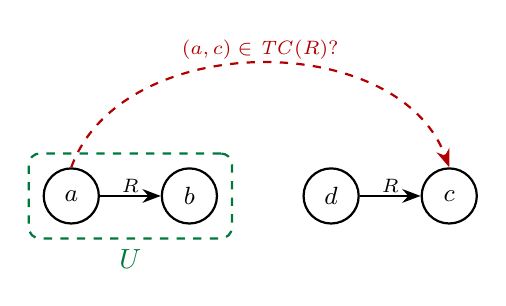
\begin{tikzpicture}[x=1cm,y=1cm]
      \node[ev] (a) at (0,0) {$a$};
      \node[ev] (b) at (1.5,0) {$b$};
      \node[ev] (d) at (3.3,0) {$d$};
      \node[ev] (c) at (4.8,0) {$c$};
      \node[draw,dashed,rounded corners,newc,thick,fit=(a)(b),inner sep=5pt,
            label={[newc]below:$U$}] {};
      \draw[arr] (a) -- node[lab,above]{$R$} (b);
      \draw[arr] (d) -- node[lab,above]{$R$} (c);
      \draw[arr,dashed,red!70!black] (a.north) to[out=70,in=110] node[lab,above]{$(a,c)\in\TC(R)$?} (c.north);
    \end{tikzpicture}
  \end{column}
  \begin{column}{0.56\textwidth}
    \footnotesize
    $(a,c)\in\TC(R)$, $R = \{(a,b),(d,c)\}$: $U = \{a, b\}$ ($b$ is reached by $(a,b)$):
    \begin{itemize}
      \item $(a,b)$: $a\in U$, so $b\in U \land \new{b\neq c}$;
      \item $(d,c)$: $d\notin U$, i.e.\ $\new{d\neq a} \land \new{d\neq b}$.
    \end{itemize}
    Each is needed: $b = c$, $d = a$ or $d = b$ makes $(a,c)$ a member. Before:
    $\mathit{distinct}(a,b,c,d)$, 7 conflicts instead of 1.
  \end{column}
  \end{columns}
\end{frame}

\begin{frame}{Grounding conflicts: the premise $S = A;B$, and the phase}
  \small
  \textbf{$S = A;B$}: the membership may be on a set $S$ equal to the join only in the current
  branch:
  \[ (a,c)\in S \qquad S = A;B \;\lor\; S = T \qquad A = \{(a,b)\} \qquad B = \{(d,c)\} \qquad
     \mathit{distinct}(a,b,c,d) \]
  $S = T$ is a model. The conflict without $S = A;B$,
  $\neg\big((a,c)\in S \land \mathit{distinct}(a,b,c,d)\big)$, excluded it too: the answer was
  \sm{unsat} (\sm{--rels-acyclic-hammer}). Now
  $\neg\big((a,c)\in S \land S = A;B \land b\neq d\big)$: \sm{sat}. Likewise $S = \TC(R)$.
  \medskip

  \textbf{Phase}: a conflict is satisfied by a merge (a disequality becomes false) or by a fresh
  member of $R$ ($R = \{..\}$ becomes false). cvc5 prefers $R = \{..\}$ true: a fresh member is
  unconstrained and leads to the next conflict with one more member, and such chains need not end
  (\sm{rel\_tc\_10\_1} with the hammer: 0.01\,s before, timeout without the preference, 0.7\,s
  with it).
  \medskip

  Regressions: \sm{rel\_join\_grounding\_key}, \sm{rel\_join\_grounding\_alias},
  \sm{rel\_tc\_grounding\_cut}, \sm{rel\_tc\_grounding\_cut\_sat}.
\end{frame}

\begin{frame}{Model construction: why \sm{sat} is correct}
  \footnotesize\vspace{-1mm}
  \textbf{How cvc5 builds the model} (\sm{collectModelValues}): every set equivalence class
  gets the union of the singletons of its known members. Relational terms are \emph{not}
  recomputed, so \sm{sat} is correct only if, when the last call is quiet, the member lists
  agree with the operators:
  \begin{center}
  \renewcommand{\arraystretch}{1.15}
  \begin{tabular}{@{}L{2.4cm}L{5.4cm}L{6.2cm}@{}}
    \toprule
    term / literal & every required member is there & every member is justified \\
    \midrule
    $\TC(R)$ & \rn{TC-Up}: the pairs of every path of $R$ &
      \rn{TC-Down} (full effort or lazy), or no unexplained member (hammer) \\
    $A;B$ & \rn{Join-Compose} & \rn{Join-Split}, or no unexplained member (hammer) \\
    \midrule
    $\cyc{R}$ & \multicolumn{2}{L{11.6cm}@{}}{quiet last call: $c \ge N$, and the model satisfies
      \rn{Unroll}$_i$ ($i < N = l$) and \rn{Split-Len}$_N$, so $s_1\to\dots\to s_N = s_1$ with
      every edge in some $\TC(R_j)$, which is the closure of $R_j$ in the model (rows above):
      $R$ has a cycle. Self-loop form: $(s,s)\in\TC(R)$.} \\
    $\neg\cyc{u}$ & \multicolumn{2}{L{11.6cm}@{}}{\rn{Register} makes $\TC(u)$ a term;
      \rn{TC-Up} puts $(a,a)$ into it for any cycle of the members of $u$; \rn{Acyclic-Down}
      refutes that: $u$ is acyclic in the model.} \\
    $\fun{R}$, $\neg\fun{R}$ & \multicolumn{2}{L{11.6cm}@{}}{\rn{Fun-UF} / \rn{Fun-Pairs}: no
      $(x,y_1),(x,y_2)$ with $y_1\ne y_2$; \rn{Not-Fun}: two such members.} \\
    \bottomrule
  \end{tabular}
  \end{center}
\end{frame}

\begin{frame}{Options and defaults}
  \footnotesize
  \begin{tabular}{@{}llL{5.2cm}@{}}
    \toprule
    option & default & effect \\
    \midrule
    \sm{--rels-functional-mode=uf|pairs} & \sm{uf} & how \sm{rel.is-functional} is used \\
    \sm{--rels-acyclic-anchor=branch|inclusion|both|none} & \sm{branch} & anchor rules \\
    \sm{--rels-acyclic-backward-chords} & off & \rn{Backward} (minimality) \\
    \sm{--rels-tc-subset} & off & closure induction \\
    \sm{--rels-tc-down-lazy} & off & \rn{TC-Down} only at last call \\
    \sm{--rels-acyclic-hammer} & off & no \rn{TC-Down} / \rn{Join-Split}; grounding conflicts \\
    \midrule
    \sm{--sets-exp} $\Rightarrow$ MiniSat & on & SAT solver unless set by the user or the
      problem is sygus-style \\
    \bottomrule
  \end{tabular}
  \bigskip

  \small
  All six new options are expert options, off or at their previous behaviour by default. The
  closure rules that need them (closure induction, lazy split, hammer) win on the benchmarks
  only in combination (next section); turning them on by default needs a broader evaluation
  (e.g.\ on cvc5/sets-and-relations-benchmarks).
\end{frame}

%=====================================================================
\section{Results}

\begin{frame}{Setup}
  \scriptsize
  \begin{tabular}{@{}lL{11.8cm}@{}}
    \toprule
    name & options (all on the files without \sm{:finite-model-find}) \\
    \midrule
    default & \sm{--finite-model-find} (as published) \\
    FMF & default + \sm{--e-matching --inst-when=full-delay --rels-acyclic-anchor=inclusion --rels-acyclic-backward-chords} \\
    noFMF & \sm{--rels-acyclic-anchor=inclusion --inst-when=full-delay --rels-acyclic-backward-chords} \\
    stop-only & default + \sm{--decision=stoponly} \\
    FMF+R & FMF + R + \sm{--rels-tc-down-lazy} \\
    noFMF+R & noFMF + R + \sm{--rels-tc-down-lazy} \\
    noFMF+H & noFMF + R + \sm{--rels-acyclic-hammer} \\
    \bottomrule
  \end{tabular}
  \smallskip

  R $=$ \sm{--prenex-quant=none --rels-tc-subset}.
  \smallskip

  \footnotesize
  \begin{itemize}
    \item 13 benchmarks with \sm{rel.cyclic} and \sm{rel.is-functional}
      (relational-solver-benchmarks \pfBench), release build of the branch (\pfCvc), \pfTimeout{} s.
    \item \textbf{Virtual portfolio}: every pair (benchmark, configuration) on its own, \pfJobs{}
      at a time; per benchmark the fastest configuration counts.
    \item \textbf{Real portfolio}: all 7 configurations started together; the first sat/unsat wins.
  \end{itemize}
  \sm{scripts/portfolio.py} runs both modes; \sm{scripts/slides/make\_figures.py} makes the
  following tables and plots.
\end{frame}

\begin{frame}{Every configuration on every benchmark (virtual portfolio)}
  \centering\tiny\setlength{\tabcolsep}{2.6pt}
  \begin{tabular}{@{}lllllllllcl@{}}
\toprule
benchmark & exp. & default & FMF & noFMF & stop-only & FMF+R & noFMF+R & noFMF+H & by & fastest \\
\midrule
sc-1-th & unsat & \tmo & \good{unsat 0.80} & \tmo & \tmo & \good{unsat 0.39} & \best{unsat 0.09} & \tmo & 3 & 0.09 s \\
sc-1-th-just-rf & unsat & \good{unsat 0.21} & \good{unsat 0.14} & \best{unsat 0.05} & \good{unsat 5.60} & \good{unsat 0.08} & \good{unsat 0.05} & \good{unsat 0.05} & 7 & 0.05 s \\
sc-1-th-no-ltts & sat & \best{sat 0.05} & \good{sat 0.09} & \textcolor{orange!80!black}{unknown} & \good{sat 0.14} & \good{sat 0.05} & \textcolor{orange!80!black}{unknown} & \tmo & 4 & 0.05 s \\
sc-2-th & unsat & \tmo & \tmo & \tmo & \tmo & \good{unsat 21.0} & \good{unsat 97.1} & \best{unsat 3.85} & 3 & 3.85 s \\
sc-2-th-just-rf & unsat & \good{unsat 1.09} & \good{unsat 0.38} & \good{unsat 0.26} & \tmo & \good{unsat 0.26} & \good{unsat 0.21} & \best{unsat 0.21} & 6 & 0.21 s \\
plsc-1-th & unsat & \tmo & \good{unsat 5.51} & \tmo & \tmo & \good{unsat 4.02} & \best{unsat 0.96} & \tmo & 3 & 0.96 s \\
plsc-1-th-just-rf & unsat & \tmo & \tmo & \tmo & \tmo & \good{unsat 0.32} & \best{unsat 0.09} & \tmo & 2 & 0.09 s \\
plsc-1-th-no-ltts & sat & \best{sat 0.09} & \good{sat 0.15} & \textcolor{orange!80!black}{unknown} & \good{sat 0.38} & \good{sat 0.09} & \textcolor{orange!80!black}{unknown} & \tmo & 4 & 0.09 s \\
plsc-2-th & unsat & \tmo & \tmo & \tmo & \tmo & \tmo & \best{unsat 76.9} & \tmo & 1 & 76.9 s \\
plsc-2-th-just-rf & unsat & \tmo & \tmo & \tmo & \tmo & \good{unsat 1.08} & \best{unsat 0.38} & \tmo & 2 & 0.38 s \\
tso-1-th & unsat & \tmo & \tmo & \tmo & \tmo & \good{unsat 294.6} & \best{unsat 7.14} & \tmo & 2 & 7.14 s \\
tso-1-th-just-rf & unsat & \tmo & \good{unsat 66.4} & \tmo & \tmo & \good{unsat 0.26} & \best{unsat 0.08} & \tmo & 3 & 0.08 s \\
tso-1-th-no-ltts & sat & \good{sat 4.35} & \tmo & \textcolor{orange!80!black}{unknown} & \tmo & \best{sat 1.27} & \tmo & \tmo & 2 & 1.27 s \\
\midrule
solved & & 5 & 7 & 2 & 3 & 12 & 10 & 3 & \multicolumn{2}{l}{\textbf{13 of 13}} \\
\bottomrule
\end{tabular}

  \medskip

  {\raggedright\scriptsize \pfTimeout{} s per run. Bold: the fastest configuration, which the
  virtual best takes. ``by'': how many configurations solve the file. \pfWrong{} wrong answers.
  The best single configuration (\pfBestSingleName) solves \pfBestSingle{}; the portfolio solves
  \textbf{\pfVirtual{} of \pfTotal}. plsc-2-th is solved by noFMF+R only.\par}
\end{frame}

\begin{frame}{The portfolio as a cactus plot}
  \centering
  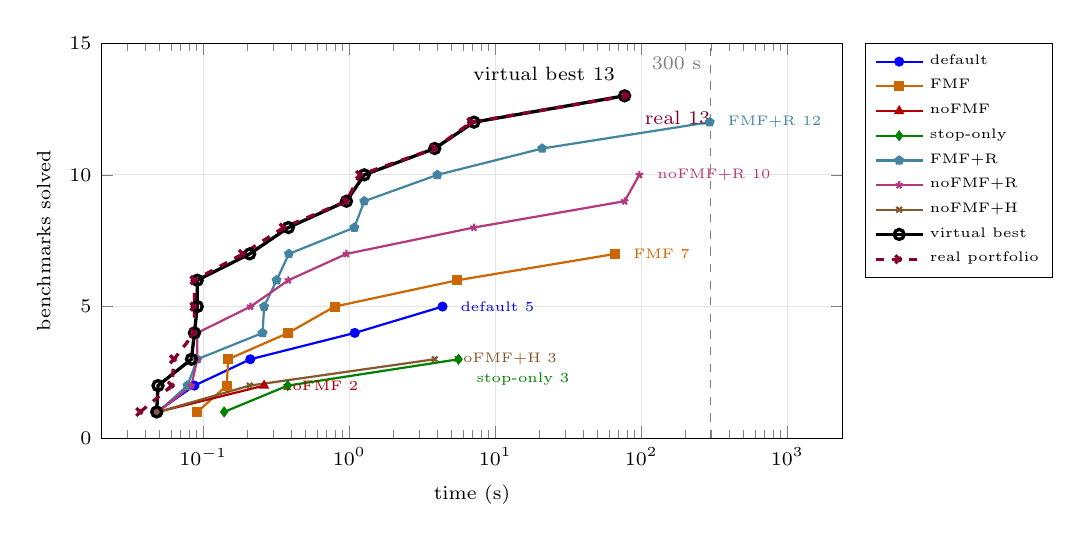
\begin{tikzpicture}
    \begin{axis}[width=11cm, height=6.6cm, xmode=log, xmin=0.02, xmax=2400,
  xlabel={time (s)}, ylabel={benchmarks solved}, ymin=0, ymax=15,
  tick label style={font=\scriptsize}, label style={font=\scriptsize},
  legend style={font=\tiny,at={(1.03,1)},anchor=north west}, legend cell align=left,
  grid=major, grid style={gray!20}]
\addplot[thick,blue,mark=*,mark size=1.4pt] coordinates {(0.048,1) (0.087,2) (0.21,3) (1.091,4) (4.352,5)};
\addlegendentry{default}
\addplot[thick,orange!80!black,mark=square*,mark size=1.4pt] coordinates {(0.091,1) (0.145,2) (0.148,3) (0.382,4) (0.795,5) (5.51,6) (66.351,7)};
\addlegendentry{FMF}
\addplot[thick,red!70!black,mark=triangle*,mark size=1.4pt] coordinates {(0.049,1) (0.261,2)};
\addlegendentry{noFMF}
\addplot[thick,green!50!black,mark=diamond*,mark size=1.4pt] coordinates {(0.139,1) (0.379,2) (5.601,3)};
\addlegendentry{stop-only}
\addplot[thick,cyan!60!black,mark=pentagon*,mark size=1.4pt] coordinates {(0.049,1) (0.078,2) (0.091,3) (0.255,4) (0.261,5) (0.318,6) (0.386,7) (1.084,8) (1.267,9) (4.019,10) (20.958,11) (294.581,12)};
\addlegendentry{FMF+R}
\addplot[thick,magenta!70!black,mark=star,mark size=1.4pt] coordinates {(0.049,1) (0.083,2) (0.091,3) (0.091,4) (0.211,5) (0.383,6) (0.957,7) (7.143,8) (76.9,9) (97.067,10)};
\addlegendentry{noFMF+R}
\addplot[thick,brown!70!black,mark=x,mark size=1.4pt] coordinates {(0.049,1) (0.208,2) (3.852,3)};
\addlegendentry{noFMF+H}
\addplot[very thick,black,mark=o,mark size=1.8pt] coordinates {(0.048,1) (0.049,2) (0.083,3) (0.087,4) (0.091,5) (0.091,6) (0.208,7) (0.383,8) (0.957,9) (1.267,10) (3.852,11) (7.143,12) (76.9,13)};
\addlegendentry{virtual best}
\addplot[very thick,purple!70!black,dashed,mark=x,mark size=2pt] coordinates {(0.037,1) (0.061,2) (0.063,3) (0.087,4) (0.087,5) (0.087,6) (0.187,7) (0.355,8) (0.955,9) (1.186,10) (3.857,11) (6.855,12) (79.549,13)};
\addlegendentry{real portfolio}
\draw[dashed,gray] (axis cs:300,0) -- (axis cs:300,15) node[pos=0.95,left,font=\scriptsize]{300 s};
\node[font=\tiny,red!70!black,anchor=west,xshift=3pt,yshift=0pt] at (axis cs:0.261,2) {noFMF 2};
\node[font=\tiny,brown!70!black,anchor=west,xshift=3pt,yshift=0pt] at (axis cs:3.852,3) {noFMF+H 3};
\node[font=\tiny,green!50!black,anchor=west,xshift=3pt,yshift=-7pt] at (axis cs:5.601,3) {stop-only 3};
\node[font=\tiny,blue,anchor=west,xshift=3pt,yshift=0pt] at (axis cs:4.352,5) {default 5};
\node[font=\tiny,orange!80!black,anchor=west,xshift=3pt,yshift=0pt] at (axis cs:66.351,7) {FMF 7};
\node[font=\tiny,magenta!70!black,anchor=west,xshift=3pt,yshift=0pt] at (axis cs:97.067,10) {noFMF+R 10};
\node[font=\tiny,cyan!60!black,anchor=west,xshift=3pt,yshift=0pt] at (axis cs:294.581,12) {FMF+R 12};
\node[font=\scriptsize,anchor=south east,yshift=2pt] at (axis cs:76.9,13) {virtual best 13};
\node[font=\scriptsize,purple!70!black,anchor=north west,xshift=3pt,yshift=-2pt] at (axis cs:79.549,13) {real 13};
\end{axis}

  \end{tikzpicture}\\
  \footnotesize Each curve: one configuration's solve times, sorted; cumulative count; final count at
  its right end. Virtual best: per file the fastest configuration. Real: all \pfNumConfigs{}
  started together.
\end{frame}

\begin{frame}{Virtual best versus real portfolio}
  \begin{columns}[T]
  \begin{column}{0.56\textwidth}
    \tiny\setlength{\tabcolsep}{3pt}
    \begin{tabular}{@{}llrrr@{}}
\toprule
benchmark & winner & VBS & real & CPU \\
\midrule
sc-1-th & noFMF+R & 0.09 s & 0.06 s & 0.4 s \\
sc-1-th-just-rf & noFMF & 0.05 s & 0.06 s & 0.3 s \\
sc-1-th-no-ltts & default & 0.05 s & 0.04 s & 0.2 s \\
sc-2-th & noFMF+H & 3.85 s & 3.86 s & 27.0 s \\
sc-2-th-just-rf & noFMF+H / noFMF+R & 0.21 s & 0.19 s & 1.2 s \\
plsc-1-th & noFMF+R & 0.96 s & 0.95 s & 6.7 s \\
plsc-1-th-just-rf & noFMF+R & 0.09 s & 0.09 s & 0.6 s \\
plsc-1-th-no-ltts & default & 0.09 s & 0.09 s & 0.6 s \\
plsc-2-th & noFMF+R & 76.9 s & 79.5 s & 556.4 s \\
plsc-2-th-just-rf & noFMF+R & 0.38 s & 0.35 s & 2.5 s \\
tso-1-th & noFMF+R & 7.14 s & 6.86 s & 48.0 s \\
tso-1-th-just-rf & noFMF+R & 0.08 s & 0.09 s & 0.5 s \\
tso-1-th-no-ltts & FMF+R & 1.27 s & 1.19 s & 7.1 s \\
\bottomrule
\end{tabular}

    \medskip

    \scriptsize Virtual: \pfVirtual{} of \pfTotal{}. Real: \pfReal{} of \pfTotal{}, with the same winner on
    \pfSame{}; real/virtual between \pfRatioMin{} and \pfRatioMax{} (median \pfRatioMed). Ratios
    below 1: the virtual runs also share the CPU (\pfJobs{} at a time).
  \end{column}
  \begin{column}{0.42\textwidth}
    \centering
    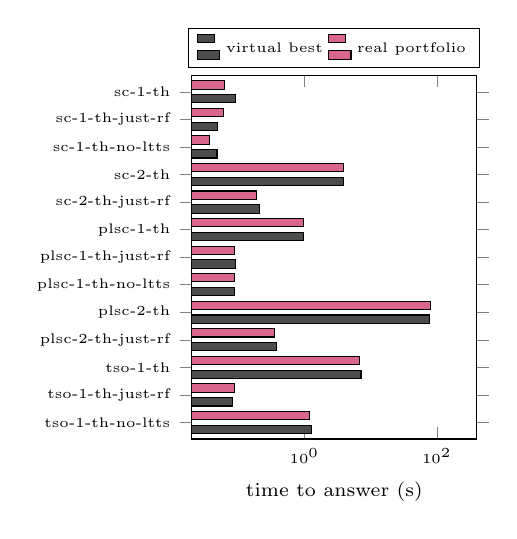
\begin{tikzpicture}
      \begin{axis}[xbar, width=5.2cm, height=6.2cm, xmode=log, log origin=infty,
  symbolic y coords={sc-1-th,sc-1-th-just-rf,sc-1-th-no-ltts,sc-2-th,sc-2-th-just-rf,plsc-1-th,plsc-1-th-just-rf,plsc-1-th-no-ltts,plsc-2-th,plsc-2-th-just-rf,tso-1-th,tso-1-th-just-rf,tso-1-th-no-ltts}, ytick=data, y dir=reverse,
  tick label style={font=\tiny}, xlabel={time to answer (s)}, xlabel style={font=\scriptsize},
  xmin=0.02, xmax=400, bar width=3pt, enlarge y limits=0.05,
  legend style={font=\tiny,at={(0.5,1.02)},anchor=south,legend columns=2}]
\addplot[fill=black!70] coordinates {(0.091,sc-1-th) (0.049,sc-1-th-just-rf) (0.048,sc-1-th-no-ltts) (3.852,sc-2-th) (0.208,sc-2-th-just-rf) (0.957,plsc-1-th) (0.091,plsc-1-th-just-rf) (0.087,plsc-1-th-no-ltts) (76.9,plsc-2-th) (0.383,plsc-2-th-just-rf) (7.143,tso-1-th) (0.083,tso-1-th-just-rf) (1.267,tso-1-th-no-ltts)};
\addplot[fill=purple!60] coordinates {(0.063,sc-1-th) (0.061,sc-1-th-just-rf) (0.037,sc-1-th-no-ltts) (3.857,sc-2-th) (0.187,sc-2-th-just-rf) (0.955,plsc-1-th) (0.087,plsc-1-th-just-rf) (0.087,plsc-1-th-no-ltts) (79.549,plsc-2-th) (0.355,plsc-2-th-just-rf) (6.855,tso-1-th) (0.087,tso-1-th-just-rf) (1.186,tso-1-th-no-ltts)};
\legend{virtual best, real portfolio}
\end{axis}

    \end{tikzpicture}\\
    \scriptsize Every real answer within \pfMaxReal{} s. plsc-2-th needs 53 s on a fast
    core, 286 s on an efficiency core.
  \end{column}
  \end{columns}
\end{frame}

\begin{frame}{Testing}
  \footnotesize
  \begin{itemize}
    \item \textbf{Regressions}: 53 new or changed files; all 443 sets, relations and bags
      regressions and all 2800 \sm{regress0} tests pass with assertions on.
    \item \textbf{Proofs}: the CPC proofs of all 84 applicable unsat relations regressions check
      with ethos; \sm{garbage\_collect.cvc} times out, as on main. The check found that
      \sm{rel.rclosure}, \sm{rel.rtclosure} were missing from the CPC signature (added).
    \item \textbf{Fuzzing} against brute force: 5\,500 random problems
      (\sm{rel.cyclic} of unions, nested either way, \sm{(not (rel.cyclic S))}, pairs forced in,
      out, or free) under five option sets: no wrong answer, no error.
    \item \textbf{Bugs found on the way, fixed in this PR}:
      \begin{itemize}
        \item the join grounding conflict refuted satisfiable branches under the hammer: first
          for lack of distinctness, then, for a membership on a set $S$ equal to the join only in
          the current branch, for lack of the premise $S = A;B$;
        \item \sm{rel.rclosure} of a union crashed debug builds, and of a variable answered
          \sm{sat} wrongly (now \sm{unknown});
        \item the MiniSat default answered \sm{unsat} wrongly with \sm{:produce-interpolants} (a
          latent issue, also on main with \sm{--sat-solver=minisat}); the default now skips
          sygus-style problems.
      \end{itemize}
    \item \textbf{CI}: formatting (clang-format 22, whole files) and the CPC/Logos check pass.
  \end{itemize}
\end{frame}

%=====================================================================
\section{Two threads under TSO}

\begin{frame}{Two new benchmarks: two threads under X86-TSO}
  \small
  \sm{tso-2-th} and \sm{tso-2-th-just-rf} (relational-solver-benchmarks \sm{ad1980d}): a candidate
  execution with \textbf{two threads}; 45 (5 in \sm{just-rf}) new template assertions over \emph{pairs} of
  communication edges, e.g.\ \sm{irr(ppo+;rf;ppo+;fr)}; the goal \sm{(not mcm)} asks for an
  execution that TSO forbids and no template excludes. Both are unsat.
  \medskip

  \textbf{Before this work} (branch of \#9):
  \begin{itemize}
    \item every configuration of the portfolio: timeout at 300 s; noFMF+R and noFMF+H: timeout
      at 3600 s;
    \item splitting \sm{(not mcm)} by the condition it violates:
  \end{itemize}
  \begin{center}\footnotesize
  \begin{tabular}{@{}llr@{}}
    \toprule
    benchmark & violated condition & result \\
    \midrule
    \sm{just-rf} & \sm{cyclic(rf)} & unsat, 0.0 s \\
    \sm{just-rf} & \sm{cyclic(ghb)}, \sm{ghb = ppo} $\cup$ \sm{rfe;sm} & \bad{timeout} \\
    \sm{tso-2-th} & atomicity, \sm{rmw} $\cap$ \sm{fre;coe} $\ne \emptyset$ & unsat, 0.1 s \\
    \sm{tso-2-th} & SC per location, \sm{cyclic(po-loc} $\cup$ \sm{rf} $\cup$ \sm{fr} $\cup$ \sm{co)} & \bad{timeout} \\
    \sm{tso-2-th} & \sm{cyclic(ghb)}, \sm{ghb = ppo} $\cup$ \sm{(rfe} $\cup$ \sm{fr} $\cup$ \sm{co);sm} & \bad{timeout} \\
    \bottomrule
  \end{tabular}
  \end{center}
\end{frame}

\begin{frame}{Why they are unsat (\sm{scripts/tso2/PROOF.md})}
  \begin{columns}[T]
  \begin{column}{0.56\textwidth}
    \footnotesize
    \begin{enumerate}
      \item \sm{po}, \sm{po}$^{-1}$ functional, \sm{po} acyclic, same-thread events
        \sm{po+}-related: \textbf{at most two chains}, and then chain $=$ thread.
      \item Take a \sm{ghb} cycle with the \textbf{fewest communication edges}; a \emph{run}
        is a maximal arc of \sm{ppo} edges. For $x \mathrel{po+} y$ in different runs of one
        chain, $(x,y)\in$ \sm{ppo} would be a shortcut; \sm{ppo} $\supseteq$ R \sm{po+} R,
        M \sm{po+} W, so $x \in W$, $y \in R$.
      \item So a chain holds \textbf{at most a write run, then a read run}: at most 4 runs.
      \item $\le 2$ communication edges: excluded by the templates.
      \item 3 or 4: a read run is left by an \sm{fr} edge (only \sm{fr} starts at a read) into the
        write run before it: $(w, w) \in$ \sm{po-loc;fr}, excluded by \sm{irr(po-loc+;fr)}.
        \sm{just-rf} has no \sm{fr}: at most 2.
    \end{enumerate}
    SC per location: the same with \sm{po-loc}.
  \end{column}
  \begin{column}{0.42\textwidth}
    \centering
    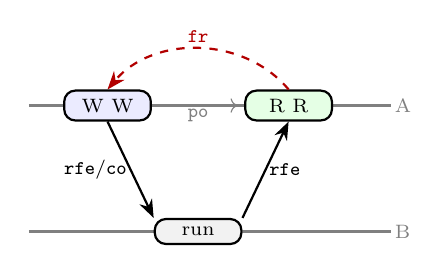
\begin{tikzpicture}[x=1cm,y=1cm]
      \draw[gray,thick] (-0.4,1.6) -- (4.2,1.6) node[right,lab]{A};
      \draw[gray,thick] (-0.4,0) -- (4.2,0) node[right,lab]{B};
      \node[box,fill=blue!8,minimum width=1.1cm] (U) at (0.6,1.6) {\scriptsize W W};
      \node[box,fill=green!10,minimum width=1.1cm] (V) at (2.9,1.6) {\scriptsize R R};
      \node[box,fill=gray!10,minimum width=1.1cm] (X) at (1.75,0) {\scriptsize run};
      \draw[->,gray] (1.25,1.6) -- node[lab,below]{\sm{po}} (2.25,1.6);
      \draw[arr] (U.south) -- node[lab,left]{\sm{rfe}/\sm{co}} (X.north west);
      \draw[arr] (X.north east) -- node[lab,right]{\sm{rfe}} (V.south);
      \draw[arr,red!70!black,dashed] (V.north) to[bend right=50] node[lab,above=1pt]{\sm{fr}} (U.north);
    \end{tikzpicture}
    \medskip

    \scriptsize $m = 3$: the read run of chain A returns by \sm{fr} to the write run before it,
    at the same address: a \sm{po-loc;fr} cycle.
  \end{column}
  \end{columns}
\end{frame}

\begin{frame}{The same argument in cvc5's witness (\sm{just-rf})}
  \begin{columns}[T]
  \begin{column}{0.44\textwidth}
    \footnotesize
    With the operands \sm{ppo} and \sm{rfe;sm}, witness edges alternate: $l = 2k+1$.
    \begin{itemize}
      \item $l = 3$, $l = 5$: \sm{irr(ppo+;rf)}, \sm{irr(ppo+;rf;ppo+;rf)}.
      \item $l \ge 7$: $s_1, s_3, s_5$ are reads, two threads, so two of them are in one thread
        (pigeonhole); \sm{po} totality orders them, and R \sm{po+} R $\subseteq$ \sm{ppo} gives a
        \rn{Chord} or a \rn{Backward} edge: a conflict on the prefix $s_1..s_5$ that holds
        \emph{for every} $l \ge 7$.
    \end{itemize}
    \textbf{Every rule this needs was in the calculus.} Given explicitly, the cycles are
    refuted in 0.1-10 s, the prefix $s_1..s_5$ with its minimality constraints in 0.1 s.
    \textbf{The search never got there.}
  \end{column}
  \begin{column}{0.54\textwidth}
    \centering
    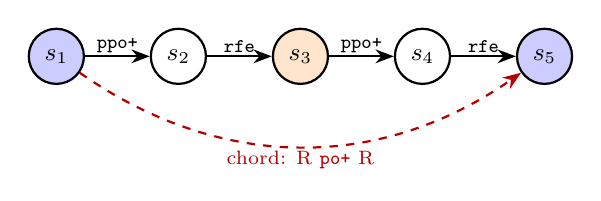
\begin{tikzpicture}[x=1.55cm,y=1cm]
      \foreach \i/\c in {1/blue,3/orange,5/blue} {
        \node[ev,fill=\c!20] (s\i) at (\i-1,0) {$s_{\i}$};
      }
      \foreach \i in {2,4} { \node[ev] (s\i) at (\i-1,0) {$s_{\i}$}; }
      \draw[arr] (s1) -- node[lab,above]{\sm{ppo+}} (s2);
      \draw[arr] (s2) -- node[lab,above]{\sm{rfe}} (s3);
      \draw[arr] (s3) -- node[lab,above]{\sm{ppo+}} (s4);
      \draw[arr] (s4) -- node[lab,above]{\sm{rfe}} (s5);
      \draw[arr,dashed,red!70!black] (s1) to[bend right=35] node[lab,below]{chord: R \sm{po+} R} (s5);
    \end{tikzpicture}
    \medskip

    \scriptsize Reads in color, one color per thread: $s_1$ and $s_5$ share a thread, so
    $(s_1, s_5)$ or $(s_5, s_1)$ is in \sm{ppo}: a chord, or a backward edge closing a shorter
    cycle. Both are forbidden by minimality.
  \end{column}
  \end{columns}
\end{frame}

\begin{frame}{Why cvc5 could not solve them (1/2): the witness search}
  \footnotesize
  \begin{enumerate}
    \item \textbf{The witness is reset by backtracking.} The witness is SAT-context dependent and
      grows by one element per full-effort round. Conflicts unrelated to the cycle undo those
      rounds, so it restarts at $s_2$: in 60 s it reached five elements twice.
    \item \textbf{Unrolling starves the quantifiers.} Kept across backtracking, the witness grows
      every round (196 elements in 60 s), every round sends a new lemma, and
      \sm{--inst-when=full-delay} waits for a quiet round that never comes: no conflict at all.
      But \sm{iden}, \sm{int}, \sm{po} totality are quantified: every template conflict needs
      instances.
    \item \textbf{The operands do not match the templates.} \sm{ghb} was flattened into the five
      components of \sm{ppo} and \sm{com;sm}; witness edges are in $\TC(\text{component})$, the
      templates speak about \sm{ppo+} $= \TC(\text{\sm{ppo}})$. (A declared \sm{ppo} is worse:
      closure induction no longer sees \sm{ppo} $\subseteq$ \sm{po+}.)
  \end{enumerate}
  \centering
  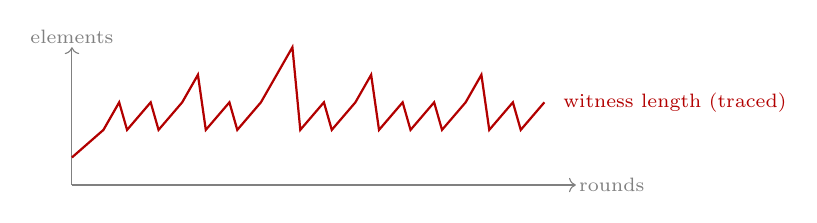
\begin{tikzpicture}[x=0.2cm,y=0.35cm]
    \draw[->,gray] (0,0) -- (32,0) node[right,lab]{rounds};
    \draw[->,gray] (0,0) -- (0,5) node[above,lab]{elements};
    \draw[thick,red!70!black] (0,1) -- (2,2) -- (3,3) -- (3.5,2) -- (5,3) -- (5.5,2) -- (7,3)
      -- (8,4) -- (8.5,2) -- (10,3) -- (10.5,2) -- (12,3) -- (13,4) -- (14,5) -- (14.5,2)
      -- (16,3) -- (16.5,2) -- (18,3) -- (19,4) -- (19.5,2) -- (21,3) -- (21.5,2) -- (23,3)
      -- (23.5,2) -- (25,3) -- (26,4) -- (26.5,2) -- (28,3) -- (28.5,2) -- (30,3);
    \node[lab,red!70!black,anchor=west] at (31,3) {witness length (traced)};
  \end{tikzpicture}
\end{frame}

\begin{frame}{Why cvc5 could not solve them (2/2): cost and a missing fact}
  \footnotesize
  \begin{enumerate}\setcounter{enumi}{3}
    \item \textbf{Quadratic lemma volume.} \sm{po} totality is instantiated for every pair of
      same-thread events, so $\TC(\text{\sm{po}})$ gets a member for almost every pair;
      \rn{TC-Up} sends one lemma per path prefix with the whole path as explanation, also for pairs
      that are already members: \textbf{134k lemmas in one minute}. The products
      \sm{Event} $\times$ \sm{Event} (in \sm{irreflexive}, \sm{int}, \sm{ext}) are composed for all
      pairs: \textbf{46k lemmas in one minute}.
    \item \textbf{A fact closure induction cannot see.} The witness of length 2,
      $(s,s) \in \TC(\text{\sm{co;sm}})$, is refuted by \sm{co;sm} $\subseteq$ \sm{co}, which holds
      because \sm{sm} $\subseteq$ \sm{iden}; but \sm{iden} is a declared constant defined by a
      quantifier. Without it \rn{TC-Down} descends forever along \sm{co} chains.
  \end{enumerate}
  \medskip
  \begin{center}
  \begin{tabular}{@{}lr@{}}
    \toprule
    one-minute run of \sm{just-rf} \sm{cyclic(ghb)}, \#9 configuration noFMF+R & \\
    \midrule
    SAT decisions / conflicts & 474\,302 / 33 \\
    witness elements unrolled & 12 \\
    time in the sets solver & 43.5 of 60 s \\
    equality-engine terms / merges & 94\,561 / 1\,420\,331 \\
    \bottomrule
  \end{tabular}
  \end{center}
\end{frame}

\begin{frame}{What \sm{cycle-ext-tso2} adds (options, off by default)}
  \scriptsize\renewcommand{\arraystretch}{1.05}
  \begin{tabular}{@{}cL{4.6cm}L{9.0cm}@{}}
    \toprule
    & option & change \\
    \midrule
    1 & \sm{cycle-keep-prefix} & continue a witness from its longest prefix \\
    2 & \sm{cycle-len-decide}, \sm{cycle-unroll-guard} & decide $l \le 2, 3, \dots$; stop unrolling there: quiet rounds \\
    3 & \sm{cycle-flatten-keep-tc} & keep a union $X$ with a term $\TC(X)$ as one operand; split $(A\cup B);C$ \\
    4 & \sm{tc-up-skip-known}, \sm{product-lazy} & no lemma for a known member; products only at last call \\
    5 & \sm{tc-subset-split} & decide $X;Y \subseteq T$ for $\TC(X;Y)$ (rule below) \\
    \bottomrule
  \end{tabular}
  \medskip

  \footnotesize\mprset{sep=1.0em}
  \begin{mathpar}
    \inferrule*[right=\rn{Subset-Split}]{\TC(X;Y) \text{ is a term}}
      {\text{decide } X;Y \subseteq T}
    \and
    \inferrule*[right=\rn{TC-Subset}]{(a,b)\in\TC(X;Y) \\ X;Y \subseteq T}{(a,b)\in T}
  \end{mathpar}
  $T = X$ if $X$ is transitive, else $\TC(X)$. So \sm{TC(co;sm)} $\subseteq$ \sm{co},
  \sm{TC(fr;sm)} $\subseteq$ \sm{TC(fr)} $=$ \sm{fr}, \sm{TC(rfe;sm)} $\subseteq$ \sm{rf}: each
  communication edge of the witness becomes a plain \sm{rf}/\sm{fr}/\sm{co} membership, and the
  templates apply. The decision is a case split, true first.
\end{frame}

\begin{frame}{Results}
  \footnotesize
  New configuration: noFMF+R $+$ the options of the previous slide and of \#11.
  \begin{center}
  \begin{tabular}{@{}lll@{}}
    \toprule
    benchmark & before & after \\
    \midrule
    \textbf{tso-2-th-just-rf} & timeout (3600 s) & \textbf{unsat, 2.5-2.9 s} (4.5 s with assertions) \\
    plsc-2-th & 53-79 s & \textbf{unsat, 11 s} \\
    tso-1-th & 6.8 s & 1.1 s \\
    tso-2-th: atomicity / SC per location & 0.1 s / timeout & 0.1 s / \textbf{29 s} \\
    tso-2-th: \sm{cyclic(ghb)} & timeout & \textbf{unsat by bounded queries} (23 min) \\
    \bottomrule
  \end{tabular}
  \end{center}
  \begin{itemize}
    \item On the 15 files: 10 of the 12 unsat files; not sc-2-th (noFMF+H solves it in 4 s) nor
      tso-2-th; not the satisfiable \sm{no-ltts} files (unsat-oriented configuration; the FMF
      configurations solve them). A portfolio with it would solve \textbf{14 of 15}.
    \item Relations regressions with all new options, assertions on: 137 runs, \textbf{no wrong
      answer}; 2 timeouts (\sm{garbage\_collect.cvc}, as on \#9, and one hammer regression).
    \item Ablation (minimal \sm{just-rf} problem): without lazy products or without length
      decisions: timeout; without keep-prefix: 3$\times$ slower.
  \end{itemize}
\end{frame}

\begin{frame}{\sm{tso-2-th} is unsat: a proof by bounded cvc5 queries}
  \begin{columns}[T]
  \begin{column}{0.5\textwidth}
    \footnotesize
    \textbf{Lemma.} A finite relation $G$ is acyclic if
    \begin{itemize}
      \item[(a)] no $n \le K$ distinct elements form a cycle $e_0 \to \dots \to e_{n-1} \to e_0$
        of $G$ edges, and
      \item[(b)] no $K$ distinct elements form a $G$ path $p_0 \to \dots \to p_{K-1}$ with no
        other $G$ edge between any two of them.
    \end{itemize}
    \emph{Proof.} Take a shortest cycle, $m$ edges. $m \le K$: (a). $m > K$: $K$ consecutive
    elements of it satisfy (b), since any other edge would shortcut the cycle or close a shorter
    one. $\square$
    \medskip

    With $G =$ \sm{ghb}, $K = 9$, on the axioms and the 44 templates of the proof (fewer
    assumptions than the benchmark), each query is a cvc5 run. With atomicity (0.1 s) and SC per
    location (29 s): \textbf{\sm{tso-2-th} is unsat}, in about 23 min of cvc5 time (15 min in
    parallel). The assertions build agrees.
  \end{column}
  \begin{column}{0.46\textwidth}
    \centering\footnotesize
    \begin{tabular}{@{}lr@{}}
      \toprule
      query & result \\
      \midrule
      (b) path of 9 elements & \textbf{unsat, 26.8 s} \\
      (a) cycles of 1, 2, 3, 4 edges & unsat, $\le$ 3.5 s \\
      5 edges & unsat, 11.9 s \\
      6 edges & unsat, 43.2 s \\
      7 edges & unsat, 95.5 s \\
      8 edges & unsat, 305.6 s \\
      9 edges & \textbf{unsat, 879.4 s} \\
      \bottomrule
    \end{tabular}
    \medskip

    \scriptsize \sm{scripts/tso2/decompose.py} writes and runs the queries;
    \sm{scripts/tso2/DECOMPOSITION.md}.
  \end{column}
  \end{columns}
\end{frame}

\begin{frame}{Why the single query does not finish: the search, not the calculus}
  \footnotesize
  \begin{itemize}
    \item \textbf{No rule is missing}: every bounded query above is decided with the existing
      rules, in seconds to minutes.
    \item \textbf{The single query must find the bound itself.} The witness is unrolled by
      iterative deepening: all lengths are refuted in one CDCL search that re-derives the same
      facts at every position, splitting on the operand of every edge and the thread of every
      element:
  \end{itemize}
  \begin{center}
  \begin{tabular}{@{}lrrrrrr@{}}
    \toprule
    length (edges) & 3 & 4 & 5 & 6 & 8 & 9 \\
    \midrule
    explicit cycle query & 0.8 s & 3.5 s & 11.9 s & 43 s & 306 s & 879 s \\
    plain-edge witness, cycles refuted up to & 3.1 s & 18.5 s & 79 s & $\approx$6 min$^*$ & $\approx$2 h$^*$ & $\approx$9 h$^*$ \\
    closure-edge witness (default) & 9.7 s & 48 s & $>$80 min & & & \\
    \bottomrule
  \end{tabular}\\[1mm]
  \scriptsize $^*$extrapolated ($\times 4.5$ per edge); with the 9-element prefix conflict, which
  covers all longer witnesses, about 11 h in total.
  \end{center}
  \begin{itemize}
    \item Explicit queries: about $\times 3$ per edge, independent. Witness: $\times 4$-6 per
      length; closure edges make it far slower.
    \item \textbf{What a solver strategy should do}: establish a length bound once with a
      length-independent query (the chord-free path), then refute each bounded length in its own
      search, possibly in parallel. That is what the decomposition does, in about 15 minutes.
  \end{itemize}
\end{frame}

%=====================================================================
\section{Summary}

\begin{frame}{Contributions}
  \begin{itemize}
    \item Two predicates for relational specifications, \sm{rel.cyclic} and
      \sm{rel.is-functional}, with API, parser, printer, type rules, rewrites, CPC declarations and
      documentation.
    \item A calculus for them in the relations solver:
      \begin{itemize}
        \item a cycle witness that is a shortest cycle of the operands' closures, unrolled
          one element per round and completed from the model;
        \item acyclicity, and anchors that connect cyclic and acyclic constraints;
        \item closure induction, which proves closure memberships without fresh elements;
        \item functionality by a skolem function;
        \item lazy and grounded closure reasoning.
      \end{itemize}
    \item A strategy that places each rule: context rules at full effort, model-dependent rules
      at last call.
    \item On the 13 litmus-template benchmarks: \textbf{13 of 13} solved by the portfolio
      (virtual and real), no wrong answer.
    \item On the two-thread TSO benchmarks (branch \sm{cycle-ext-tso2}): a hand proof of both;
      seven prototype options that make the witness search work; \sm{tso-2-th-just-rf} unsat in
      3 s; \sm{tso-2-th} unsat by bounded cvc5 queries (23 min), not yet as a single query.
  \end{itemize}
\end{frame}

\begin{frame}{Where to find it}
  \small
  \begin{itemize}
    \item PR to cvc5 main: \sm{mudathirmahgoub/cvc5\#17} (branch \sm{cycle-ext-cyclic}); the same
      branch is \sm{rachelcleaveland/cvc5\#9}, stacked on the earlier \sm{cycle-ext} PRs.
    \item Two-thread TSO: branch \sm{cycle-ext-tso2} (on top of \sm{rachelcleaveland/cvc5\#11});
      proof, notes and test files in \sm{scripts/tso2/}.
    \item Benchmarks: \sm{rachelcleaveland/relational-solver-benchmarks}, directories
      \sm{benchmarks-ltts} and \sm{benchmarks-ltts-nofmf}.
    \item Temporary, to be deleted before merging: \sm{scripts/} (portfolio runner, ablation,
      comparison, converters) and \sm{scripts/slides/} (this deck, its figure generator and the
      run data).
    \item Rebuild the deck: \sm{cd scripts/slides; python3 make\_figures.py data/final-300s
      figures; pdflatex relations-pr.tex}.
  \end{itemize}
\end{frame}

\end{document}
